\label{ch:galerkin}

\section{Introduction}

We consider two-dimensional correlated Brownian motion with absorbing boundaries:
\begin{align}
  X(t) &= x_0 + \mu_x t + \sigma_x W_x(t) &a_x &\leq X(t) \leq b_x   \label{eq:X} \\
  Y(t) &= y_0 + \mu_y t + \sigma_y W_y(t) &a_y &\leq Y(t) \leq b_y   \label{eq:Y} 
\end{align}
where $W_i$ are standard Brownian motions with
$\mbox{Cov}(W_1(t), W_2(t)) = \rho t$. We find the below probability
for $(X(t), Y(t))$ and the random variables
$M_X(t)=\max_{0\leq s\leq t}X(t),$ $m_X(t)=\min_{0\leq s\leq t}X(t),$
$M_Y(t)=\max_{0\leq s\leq t}Y(t),$ $m_Y(t)=\min_{0\leq s\leq t}Y(t)$
\begin{align}
  \mbox{Pr}\left( \left. \begin{array}{ll}
                           X(t) \leq x_t, & Y(t) \leq y_t, \\
                           M_X(t) \leq b_x, & M_Y(t) \leq b_x, \\
                           m_X(t) \geq a_x, & m_Y(t) \geq a_y,
                         \end{array} \right| X(0) = x_0, Y(0) = y_0, \theta \right)
                                              \label{eq:CDF}
\end{align}
with $\theta := (\mu_x, \mu_y, \sigma_x, \sigma_y, \rho).$ This
probability can be expressed as the integral
\[
  \displaystyle \int_{a_x}^{x_t} \displaystyle \int_{a_y}^{y_t} q(x,y,t) dx\,dy,
\]
where $q(x,y,t)$ is the solution to the Fokker-Planck equation
\cite{oksendal2013stochastic}:
\begin{align}
  \displaystyle \frac{\partial}{\partial t'} q(x,y,t') &= -\mu_x \frac{\partial}{\partial x}q(x,y,t')
                                         - \mu_y \frac{\partial}{\partial y}q(x,y,t')
                                         + \frac{1}{2}\sigma_x^2 \frac{\partial^2}{\partial x^2}q(x,y,t')
                                         + \rho\sigma_x\sigma_y \frac{\partial^2}{\partial x \partial y}q(x,y,t')
                                         + \frac{1}{2}\sigma_y^2 \frac{\partial^2}{\partial y^2}q(x,y,t'),
  \label{eq:1} \\
  q(a_x, y,t') &= q(b_x,y,t') = q(x,a_y,t') = q(x,b_y,t') = 0, \label{eq:2} \\
   0 &< t' \leq t. \nonumber
\end{align}
Differentiating $q(x,y,t)$ with respect to the boundaries produces the
transition density of a particle beginning and ending at the points
$(X(0), Y(0))$ and $(X(t), Y(t))$, respectively, while
attaining the minima $a_x/a_y$ and maxima $b_x/b_y$ in each coordinate
direction. This transition density is equivalent to the joint density
for $(X(t), Y(t), m_X(t), M_X(t), m_Y(t), M_Y(t))| X(0)=x_0, Y(0)=y_0$,
which we denote as $f(x,y,a_x,b_x,a_y,b_y)$:
\begin{align}
  \frac{\partial^4}{\partial a_x \partial b_x \partial a_y \partial b_y} q(x,y,t) = f(x,y,a_x,b_x,a_y,b_y).
  \label{eq:pdf}
\end{align}
Probability functions similar to (\ref{eq:CDF}) with less than all
four boundaries have been used in computing first passage times
\cite{kou2016first, sacerdote2016first}, with application to
structural models in credit risk and default correlations
\cite{haworth2008modelling, ching2014correlated}. \cite{he1998double}
use variants of (\ref{eq:pdf}) with respect to some of the boundaries
to price financial derivative instruments whose payoff depends on
\textit{some} of the observed maxima/minima. \cite{rodriguez2012} use
a full likelihood-based (Bayesian) approach to estimate volatility in
\textit{univariate} financial timeseries where open, closing, highest,
and lowest prices are included. Their work fits into a body of
literature and collection of techniques by practitioners where the
observed range of prices is used to make similar estimates. In this
chapter we will provide an efficient numerical method necessary for
carrying out inferential procedures with correlated financial
timeseries in the bivariate setting.

Closed-form solutions to (\ref{eq:1}) - (\ref{eq:2}) are available for
some parameter regimes. When $\rho = 0$, the transition density of the
process is the solution to a well-understood Sturm-Liouville problem
where the eigenfunctions of the differential operator are sine
functions. When $a_x = -\infty$ and $b_x = \infty$, the method of
images can be used to enforce the remaining boundaries. For either
$a_x, a_y = -\infty$ or $b_x, b_y = \infty$, eigenfunctions of the
Fokker-Plank equation can be found in radial coordinates. Both of
these techniques are used and detailed by
\cite{he1998double}. However, to the best of our knowledge, there is
no closed-form solution to the general problem in (\ref{eq:1}) -
(\ref{eq:2}). This also limits the available ways to compute
(\ref{eq:pdf}), with the most straightforward approach being finite
difference with respect to the boundary conditions. This, however,
requires one to solve Fokker-Planck equation (\ref{eq:1}) - (\ref{eq:2})
accurately for at least 16 slightly different sets of boundaries and
combine the results with numerical differentiation to evaluate the
density function for a just single observation (see Section
\ref{sec:likelihood-calc}), motivating the need for an efficient
numerical method to solve (\ref{eq:1}) - (\ref{eq:2}).

For non-zero correlation, it is still possible to approach the general
problem by proposing a biorthogonal expansion in time and space
(\cite{risken1989fokker-planck}, sections 6.2), where the
eigenfunctions for the differential operator are approximated by the
eigenvectors of a linear system obtained using a truncated expansion
based on a set of separable basis function, each of which is a product
of two sine functions (one in each dimension) satisfying the boundary
conditions. However, a drawback of this out-of-the-box solution is
that the system matrix for the corresponding eigenvalue problem is
dense. Additionally, for nonzero $\rho$, it is necessary to have a
large number of basis elements for an accurate approximation. The
denseness and size of the resultant system makes the
expansion a slow, if not unfeasible, solution. An alternative is to
use a finite difference scheme to directly solve the evolution problem
after suitable transformations. However, both of these methods need a
high degree of numerical resolution to produce practically useful
approximations of the transition density. We conjecture that for the
trigonometric series expansion, inefficiencies arise from using a
separable representation for a differential operator that is
intrinsically correlated in the two dimensions; for the finite
difference approach, the problem is twofold as the method introduces
numerical diffusion in the initial condition and it also uses a
separable approximation for the differential operator.

In the following two chapters we propose robust and efficient
solutions to the problems (\ref{eq:1}) - (\ref{eq:2}) and
(\ref{eq:pdf}) in two distinct parameter regimes. The twofold solution
is obtained by combining a small-time analytic solution with a
Galerkin discretization based on basis functions that are
correlated.

This chapter describes the Galkerin discretization, which directly
takes into account the correlation parameter present in the
differential operator in order to efficiently represent an analytic
small-time solution and propagate it forward in time. We apply our
computational method to estimate equation parameters with a maximum
likelihood approach in settings where the model assumptions of
constant $(\mu_x, \mu_y, \sigma_x, \sigma_y, \rho)$ and Brownian
motion driving stochastic evolution are appropriate. Section
\ref{sec:approximate-sols} outlines some methods we considered for
this problem. Section \ref{sec:semidiscrete-galerkin} describes the
Galerkin method we implemented. Section [] includes our numerical
experiments.


\section{Approximate Numerical Solutions} \label{sec:approximate-sols}
Before considering solutions to the full Fokker-Planck equation
(\ref{eq:1}) - (\ref{eq:2}), we simplify the PDE by proposing a series
of transformations to standardize the problem. The first transformation
\begin{align}
  T_{(1)} : q(x,y,t) &\to p(x,y,t)
\end{align}
scales and decomposes the solution while preserving the initial and
boundary conditions while getting rid of the advection terms in the
differential operator. $T_1$ is defined as
\begin{align}
  T_{(1)}: p(x,y,t) &= \exp(\alpha x + \beta y + \gamma t) q\left( x(b_x - a_x) + a_x, \,\, y(b_y - a_y) + a_y, \,\, t \right), \label{eq:q-to-p}
\end{align}
where


\begin{align*}
  \alpha &= -\frac{\mu_x}{\sigma_x^2} - \frac{\rho}{\sigma_x\sigma_y(1-\rho^2)}\left( -\frac{\mu_y}{\sigma_y^2} + \frac{\mu_x \rho}{\sigma_x \sigma_y} \right), \\
  \beta &= \left( -\frac{\mu_y}{\sigma_y^2} + \frac{\mu_x \rho}{\sigma_x \sigma_y} \right), \\
  \gamma &= \frac{1}{2}\left( \frac{\sigma_x}{(b_x-a_x)} \right)^2 \alpha^2 + \frac{1}{2}\left(\frac{\sigma_y}{(b_y-a_y)}\right)^2 \beta^2 + \alpha\beta.
\end{align*}
This new formula satisfies the \textit{pure diffusion} equation:
\begin{equation}
  \frac{\partial}{\partial t} p(x,y,t) = \mathcal{L}_1 p(x,y,t),\quad (x,y) \in (0,1) \times (0,1) := \Omega_1 \label{eq:qq}
\end{equation}
subject to the constraints
\begin{align}
  p(x,y,t) &=0, & \mbox{ for } & (x,y) \in \{ x | x = 0\} \cup \{ y | y = 0\} \cup \{ x | x = 1\} \cup \{ y | y = 1\}, \nonumber \\
  p(x,y,0) &= \delta\left( x - \frac{x_0-a_x}{b_x - a_x} \right) \delta\left(y-\frac{y_0 - a_y}{b_y - a_y}\right), \nonumber
\end{align}
where the differential operator $\mathcal{L}_1$ takes the form
\[
  \mathcal{L}_1 = \frac{1}{2} \tau_x^2 \frac{\partial^2}{\partial x^2}
  + \rho\tau_x\tau_y \frac{\partial^2}{\partial x \partial y} + \frac{1}{2}\tau_y^2 \frac{\partial^2}{\partial y^2},
  % \left(  \right)^2
  %                                                   \frac{\partial^2}{\partial x^2}p(x,y,t) + \rho\left( \frac{\sigma_x}{(b_x-a_x)} \right)\left( \frac{\sigma_y}{(b_y-a_y)} \right)
  %                                                   \frac{\partial^2}{\partial x \partial y}p(x,y,t) +
  %                                        \frac{1}{2}\left( \frac{\sigma_y}{(b_y-a_y)} \right)^2 \frac{\partial^2}{\partial y^2}p(x,y,t) , \label{eq:qq} \\
\]
with $\tau_x = \frac{\sigma_x}{(b_x-a_x)}$,
$\tau_y = \frac{\sigma_y}{(b_y-a_y)}$.  Note here that under this
transformation $\rho$ remains the same as in the original
problem.

Next, we \textit{normalize} the diffusion equation (\ref{eq:qq}) with the transformation
\begin{align}
  T_{(2)}: p(x,y,t) &\to p(\tilde{x}, \tilde{y}, \tilde{t}),
\end{align}
defined with the coordinate transformation
\begin{align}
  \tilde{x} &= x\cdot \Indicator{ \max\left\{\tau_x^2, \tau_y^2 \right\} = \tau_x^2} + y\cdot \Indicator{ \max\left\{\tau_x^2, \tau_y^2 \right\} = \tau_y^2}, \\
  \tilde{y} &= y\cdot \Indicator{ \max\left\{\tau_x^2, \tau_y^2 \right\} = \tau_x^2} + x\cdot \Indicator{ \max\left\{\tau_x^2, \tau_y^2 \right\} = \tau_y^2}, \\
  \tilde{t} &= t\cdot \max\left\{\tau_x^2, \tau_y^2 \right\}.
\end{align}
The differential problem under $T_{(2)}$ now takes on the
\textit{normalized form} (from hereon referred to as the
\textit{normalized problem}):
\begin{align}
  \frac{\partial}{\partial \tilde{t}} p(\tilde{x},\tilde{y},\tilde{t}) &= \mathcal{L}_2 p(\tilde{x},\tilde{y},\tilde{y}), & (\tilde{x}, \tilde{y}) \in (0,1) \times (0,1) := \Omega_2 \label{eq:qqq} \\
  \mathcal{L}_2 &= \frac{1}{2} \frac{\partial^2}{\partial \tilde{x}^2} + \rho \sigma_{\tilde{y}} \frac{\partial^2}{\partial \tilde{x} \partial \tilde{y}} + \frac{1}{2} \sigma^2_{\tilde{y}} \frac{\partial^2}{\partial \tilde{y}^2},
\end{align}
with
$\sigma_{\tilde{y}} = \min\left\{ \tau_x/\tau_y, \tau_y/\tau_x
\right\}$ subject to the IC/BCs:
\begin{align}
  p(\tilde{x},\tilde{y},\tilde{t}) &=0,  \mbox{ for }  (\tilde{x},\tilde{y}) \in \{ \tilde{x} | \tilde{x} = 0\} \cup \{ \tilde{y} | \tilde{y} = 0\} \cup \{ \tilde{x} | \tilde{x} = 1\} \cup \{ \tilde{y} | \tilde{y} = 1\}, \nonumber \\
  p(\tilde{x},\tilde{y},0) &= \delta\left( \tilde{x} - \left\{\frac{x_0-a_x}{b_x - a_x}\cdot \Indicator{ \max\left\{\tau_x^2, \tau_y^2 \right\} = \tau_x^2} + \frac{y_0-a_y}{b_y - a_y}\cdot \Indicator{ \max\left\{\tau_x^2, \tau_y^2 \right\} = \tau_y^2} \right\} \right) \\
  &\quad \times \delta\left( \tilde{y} - \left\{\frac{y_0-a_y}{b_y - a_y}\cdot \Indicator{ \max\left\{\tau_x^2, \tau_y^2 \right\} = \tau_x^2} + \frac{x_0-a_x}{b_x - a_x}\cdot \Indicator{ \max\left\{\tau_x^2, \tau_y^2 \right\} = \tau_y^2} \right\} \right). \nonumber
\end{align}
As seen above, the computational domain under $T_{(2)}$ remains the
unit square. However, the diffusion coefficient in the principal
$\tilde{x}$-direction is always unity, while
$\sigma_{\tilde{y}} \leq 1$. The time for evaluating the final
condition is scaled by either $\tau_x^2$ or $\tau_y^2$, while the
correlation coefficient remains the same. The initial condition
location parameters, $\sigma_{\tilde{y}}$, as well as the time of the
final condition $\tilde{t}$ are all functions of the boundary
parameters $(a_x, b_x, a_y, b_y)$. Without loss of generality, we will
concentrate on the solution of the normalized problem (\ref{eq:qqq})
in terms of the diffusion parameters
$(\tilde{t}, \sigma_{\tilde{y}}, \rho)$.

\subsection{Density Calculation} \label{sec:likelihood-calc}
Recalling problem (\ref{eq:pdf}), to compute the density we are
interested in, we must take derivatives of the solution $p(x,y,t)$
with respect to the boundary parameters $(a_x, b_x, a_y,
b_y)$. Because the approximate solutions we will consider below are
functions of the parameters without explicit analytic form,
$\frac{\partial^4}{\partial a_x\partial b_x \partial a_y \partial
  b_y}p(x,y,t)$ must be computed numerically using a finite difference
approximation. We must therefore find the solution for each of the
sixteen perturbed problems
\[
  p(x,y,t | a_x \pm \epsilon, b_x \pm \epsilon, a_y \pm \epsilon, b_y
  \pm \epsilon).
\]
The derivative of $p$ with respect to the 4 boundaries is approximated
as
\begin{eqnarray*}
& & \frac{\partial^4}{\partial a_x \partial b_x \partial a_y \partial b_y} p(x, y, t) 
\nonumber \\
& & \hspace*{0.5cm} \approx \frac{\displaystyle \sum_{k_1, k_2, k_3, k_4 = \pm 1}
c_{\{ k_1, k_2, k_3, k_4 \} } p(\left. x, y, t \right| a_x+k_1 \varepsilon, b_x+k_2 \varepsilon, 
a_y+k_3 \varepsilon, b_y+k_4 \varepsilon) }{(2 \varepsilon )^4} 
\nonumber
\end{eqnarray*}
The finite difference approximation, however, introduces fundamental
limitations for the type of approximation that can be used and the
degree of accuracy admissible for this problem.

Consider an approximate solution $p^{(k)}(\left. x, y, t \right| b)$
where we have included parameter $b $ explicitly as a simplified
notation for $[a_x, b_x]$ and $[a_y, b_y]$ and we assume that the
approximation approaches the true solution as $k \to \infty$. In
general, the truncation error can be represented as
\begin{align}
  p^{(k)}(x,y,t | b) - p(x,y,t | b) = \left( \frac{1}{k}
  \right)^{\alpha} \mbox{F}_{reg}(b) + \left( \frac{1}{k}
  \right)^{\beta}\mbox{F}_{irreg}(b) + \varepsilon_{mach}F_{round}(b), \label{eq:trunc-error}
\end{align}
for some $\alpha, \beta > 0$; $(1/k)^{\alpha} \mbox{F}_{reg}(b) $ is
the regular part of the truncation error,
$(1/k)^{\beta} \mbox{F}_{irreg}(b) $ is the irregular part of the
truncation error, and $\varepsilon_{mach} \mbox{F}_{round}(b) $ is the
effect of round-off errors with $\varepsilon_{mach} \sim 10^{-16}$
denoting the machine epsilon for IEEE double precision system.

Note that when expressed using the chain rule, both
$\displaystyle \frac{\partial}{\partial a_x}$ and
$\displaystyle \frac{\partial}{\partial b_x}$ contain
$\displaystyle \frac{\partial}{\partial b}$. As a result,
$\displaystyle \frac{\partial^2 }{\partial a_x \partial b_x} $ leads
to $\displaystyle \frac{\partial^2 }{\partial b^2} $. Although in the
discussion below, for simplicity, we only illustrate the numerical
differentiation on the first derivative, keep in mind that it is the
second derivative that is more relevant in the calculation of
$\displaystyle \frac{\partial^4}{\partial a_x \partial b_x \partial
  a_y \partial b_y} p(x, y, t) $.

The coefficient, $\mbox{F}_{reg}(b) $, of the regular part of
truncation error is a smooth function of $b$ with derivative $= O(1)$.
The coefficient, $\mbox{F}_{round}(b) $, in the effect of round-off
errors, behaves virtually like a random variable, discontinuous in
$b$.  For the irregular part of truncation error, the coefficient
$\mbox{F}_{irreg}(b) $ can be thought of in general as continuous in
$b$ but not smooth in $b$ where the derivative has
discontinuities. Linear interpolation, for example, introduces this
kind of irregular truncation error. Based on the expression we wrote
out above for the finite difference solution, applying the numerical
differentiation with step $\varepsilon$ yields:
\begin{eqnarray}
  & & \frac{p^{(k)}(\left. x, y, t \right| b+\varepsilon)-p^{(k)}(\left. x, y, t \right| b -\varepsilon)}{2 \varepsilon} \nonumber \\
  & & \hspace*{1cm} =  \frac{\partial }{\partial b} p(\left. x, y, t \right| b) + O(\varepsilon^2)
      + \left(\frac{1}{k}\right)^{\alpha} \frac{\mbox{F}_{reg}(b+\varepsilon)-\mbox{F}_{reg}(b-\varepsilon)}{2 \varepsilon}  \nonumber \\
  & & \hspace*{1cm} + \left(\frac{1}{k}\right)^{\beta} \frac{\mbox{F}_{irreg}(b+\varepsilon)-\mbox{F}_{irreg}(b-\varepsilon)}{2 \varepsilon}
      + \varepsilon_{mach} \frac{\mbox{F}_{round}(b+\varepsilon)-\mbox{F}_{round}(b-\varepsilon)}{2 \varepsilon}  \nonumber
\end{eqnarray}
In the equation above, as the step in the numerical differentiation is
refined, the first line of the RHS is well behaved, converging to the
true value $\frac{\partial }{\partial b} p(\left. x, y, t \right| b)$
as $\varepsilon \rightarrow 0$.  The second line of RHS, however, is
problematic. As $\varepsilon \rightarrow 0$, the contribution from
round-off error blows up to infinity
\[
  \varepsilon_{mach}
  \frac{\mbox{F}_{round}(b+\varepsilon)-\mbox{F}_{round}(b-\varepsilon)}{2
    \varepsilon} = O\left(\frac{\varepsilon_{mach}}{\varepsilon}
  \right) \longrightarrow \infty \;\;\;\; \mbox{as } \varepsilon
  \rightarrow 0
\]
For a fourth-order derivative, the error
contribution of finite machine precision becomes
$O(\varepsilon_{mach}/\varepsilon^4)$ and a step size as big as
$\varepsilon \sim 10^{-4}$ produces errors $O(1)$. This is
catastrophic in instances where values of the density are smaller than 1.

The contribution from the irregular part of truncation error can also
be problematic if the finite difference approximation of the
derivative of $F_{irreg}(b)$ is $O(k^\beta/\varepsilon)$; we will show
that this is the case for the finite difference method.  As a
consequence of both machine precision and possible irregular
truncation errors, we observe that there is a fundamental restriction
of the size of finite difference steps $\varepsilon$ we can use in the
numerical methods below.

\subsection{Eigenfunction Expansion} \label{sec:eigenfunction}
Following Section 6.2 of \cite{risken1989fokker-planck}, we may use
the biorthogonal decomposition of the solution as a sum of
eigenfunctions and time-dependent coefficients determined by eigenvalues:
\begin{equation}
  p(x,y,t) =  \sum_\nu h_\nu \phi_\nu (x, y) e^{-\lambda_\nu t}, \label{eq:biorthogonal}
\end{equation}
where $h_\nu$ is the coefficient of $\phi_\nu(x, y)$ is the
eigenfunction expansion of $p(x,y,0)$. Because the differential
operator $\mathcal{L}$ is self-adjoint, the family of eigenfunctions
is complete in the Hilbert space $L_2(\Omega)$. Moreover, the
eigenvalues are bounded below by a positive constant $c$, so that the
solution behaves as expected (see section 6.3 of
\cite{risken1989fokker-planck}).

Since we require $\phi_\nu(x,y)$ to be zero on the boundaries, we
approximate the eigenfunction using a finite set of orthogonal basis
functions satisfying boundary conditions, i.e., a finite sequence of
sines,
\[
  \phi_\nu(x,y) = \sum_{l=1}^L \sum_{m=1}^M c_{l,m, \nu}
  \sin\left(2\pi\, l\, x \right) \sin\left(2\pi\, m\, y \right) := \Psi(x,y)^T c_\nu,
\]
where we have truncated the infinite series for some suitably large
$L$ and $M$ and defined
\begin{align*}
  \psi_{l,m}(x,y) &= \sin\left(2\pi\, l\, x \right)
                         \sin\left(2\pi\, m\, y \right), \\
  \Psi(x,y) &= (\psi_{1,1}(x,y), \ldots, \psi_{L,M}(x,y))^T, \\
  c_\nu &= (c_{1,1,\nu}, \ldots, c_{L,M,\nu})^T.
\end{align*}
The biorthogonal representation (\ref{eq:biorthogonal}) leads to the
eigenvalue problem
\begin{equation}
  \mathcal{L} \phi_\nu = -\lambda_\nu \phi_\nu, \label{eq:eigenproblem}
\end{equation}
where $\mathcal{L}$ is the differential operator in the normalized
Fokker-Planck equation. Applying $L$ to the basis function expansion
of $\phi_v $ and again approximating the result using the finite set
of basis functions yields
\[
  \mathcal{L}\phi_\nu = \mathcal{L}(\Psi(x,y)^T c_\nu) =
  \mathcal{L}(\Psi(x,y)^T) c_\nu = (A \Psi(x,y))^T c_\nu,
\] 
where $A$ is a matrix analytic in $(\tau_x, \tau_y, \rho)$. In the
last part of the equation above, we have truncated the infinite sine
series expansion of $L \psi_{l, m}(x, y)$. In the case where
$\rho = 0$, $A$ is diagonal because $\left\{ \psi_{l,m}(x,y) \right\}$
are the eigenfunctions to $\mathcal{L}$. When $\rho \neq 0$, $A$ is no
longer diagonal and is in fact dense. % The dense structure of matrix
% $A$ is caused by the mixing terms
% \[
%   \frac{\partial^2}{\partial x \partial y} \sin\left(2\pi\, l\,
%     x\right) \sin\left(2\pi\, m\, y\right) = (2\pi\, l)(2\pi\, m)
%   \cos\left(2\pi\, l\, x\right) \cos\left(2\pi\, m\, y\right)
% \]
% being the products of cosine functions, which have an inefficient
% sine series representation [CITE].
Substituting the linear representation
of $\mathcal{L}\phi_\nu$ into the eigenvalue problem
(\ref{eq:eigenproblem}), we arrive at the matrix eigenvalue problem
\[
  \Psi(x,y)^T A^T c_\nu = -\lambda_\nu \Psi(x,y)^T c_\nu
  \quad \Leftrightarrow \quad A^T c_\nu = -\lambda_\nu c_\nu
\]
whose solution gives the family of orthonormal eigenfunctions. As
mentioned already, the efficiency of this approach is dependent on the
cost of solving the eigenvalue problem
$A^T c_\nu = -\lambda_\nu c_\nu$.  With all of the eigenpairs
$(c_\nu, \lambda_\nu)$, the approximate solution is then
\[
  p(x,y,t) \approx \Psi(x,y)^T \sum_{\nu} h_\nu c_\nu e^{-\lambda_\nu t}.
\]

In terms of density calculations for
$\frac{\partial^4 p(x,y,t)}{\partial a_x \partial b_x, \partial
  a_y \partial b_y}$, the eigenfunction expansion does not suffer from
having irregular truncation errors, because $A$ is analytic in the
diffusion parameters and the eigenpairs $(\lambda_\nu, c_\nu)$ inherit
this property (see Theorems 7 and 8 of Chapter 9 in
\cite{lax2007linear-algebra}). However, because a good working
approximation of $p(x,y,t)$ requires many terms in the expansion, and
because each resultant system matrix is dense, repeated computation of
the eigenproblem for the density calculation is unfeasible.

\subsection{Finite Difference} \label{sec:finite-difference} A finite
difference method which approximates the spatial derivatives in
problem (\ref{eq:qq}) requires the solution a system of differential
equations
\begin{align}
  \dot{c}(t)= B c(t) &\Rightarrow& c(t) = \exp\left( Bt \right)c(0) \label{eq:eigenproblem-fd}, 
\end{align}
which reduces to the eigenvalue decomposition of a matrix $B$. Here,
$c(t)$ is a vector consisting of values of the solution in
(\ref{eq:qq}) on a set of grid points over $\Omega$ at time $t$, and
the product $Bc(t)$ approximates $\mathcal{L}p(x,y,t)$. The system
matrix $B$ is dependent on the discretization scheme used to
approximate $\mathcal{L}$. Using a central-in-space scheme over a
\textbf{regular} grid on $\Omega$ with $\Delta x = \Delta y = h$,
\[ B = \frac{1}{2}\tau_x^2 \frac{1}{h^2}B_{x,x} +
  \rho\tau_x\tau_y \frac{1}{4h^2}B_{x,y} + \frac{1}{2}\tau_y^2
  \frac{1}{h^2}B_{y,y},
\]
where each of the matrices $B_{x,x}, B_{x,y}, B_{y,y}$ approximate
$\frac{\partial^2}{\partial x^2}, \frac{\partial^2}{\partial
  x \partial y}, \frac{\partial^2}{\partial y^2}$, respectively.
% For
% example, using $c_{l, m}(t) $ to denote the approximation of the
% solution at grid point $(x_l, y_m)$, and assembling vector $c(t)$
% using the index scheme $c_{l, m}(t) \rightarrow c_k(t)$ with
% $k= (l-1) M + m$, we can approximate the operator
% $\frac{\partial^2 }{\partial x^2} $ as
% \begin{align*}
%   \frac{1}{2}\tau_x^2 \frac{\partial^2}{\partial x^2} p(x_l,y_m,t) \approx \frac{1}{2}\tau_x^2 \left( \frac{c_{l+1,m}(t) - 2c_{l,m}(t) + c_{l-1,m}(t)}{h^2} \right) = \frac{1}{2}\tau_x^2 \frac{1}{h^2}A_{x,x}[k,] c(t) 
% \end{align*}
% where $A_{x,x}[k,]$ is the $k^{th}$ row of $A_{x,x}$. Similarly,
% \begin{align*}
%   \rho\tau_x\tau_y \frac{\partial^2}{\partial x \partial y} p(x_l,y_m,t) \approx \rho\tau_x\tau_y \left( \frac{c_{l+1,m+1}(t) - c_{l+1,m-1}(t) - c_{l-1,m+1}(t) + c_{l-1,m-1}(t)}{4h^2} \right) = \rho\tau_x\tau_y \frac{1}{4h^2}A_{x,y}[k,] c(t) 
% \end{align*}
It should be noted here that a regular grid approach with a constant
$h$ independent of parameters is appealing, because it allows us to
construct once and store the matrices $B_{x,x}, B_{x,y}, B_{y,y}$,
which saves valuable computational resources if we are to solve the
finite difference eigenproblem (\ref{eq:eigenproblem-fd}) repeatedly
for different parameter values $(\tau_x,\tau_y,\rho)$.

Unlike the system matrix for the trigonometric expansion, the system
matrix $B$ here is sparse: each row of $(B_{x,x}, B_{x,y}, B_{y,y})$
is composed of all zeros except for three or four entries. This
structure does not change as $h \to 0$. The eigenvalue problem is
therefore much cheaper to solve.

However, the fundamental limitation of using a finite difference
method is that it introduces irregular truncation error, because of
the linear interpolation necessary for function arguments not on grid
points. Referring to the notation in (\ref{eq:trunc-error}), and
setting $k := 1/h$, the interpolation error introduced by a finite
difference scheme at position $b$ for the boundary parameters using
step $h$ has the general form of
$$\mbox{Interpolation error } = O(h^2) (1-\mbox{rem}(b/h,1)) \mbox{rem}(b/h,1)$$ 
The coefficient part
$\mbox{F}_{irreg}(b) = (1-\mbox{rem}(b/h,1)) \mbox{rem}(b/h,1) $ is
continuous in $b$ but not differentiable. Its first derivative has the
behavior of
$$ \frac{\partial }{\partial b} \mbox{F}_{irreg}(b) =  \frac{1}{h} \left(1-2\mbox{rem}(b/h,1) \right).$$ The contribution from the irregular part of truncation error is 
$$ h^2 \frac{\mbox{F}_{irreg}(b+\varepsilon)-\mbox{F}_{irreg}(b-\varepsilon)}{2 \varepsilon}  = 
O\left(\frac{h^2}{\max(\varepsilon, h)} \right) $$ 
In the second order numerical differentiation, however, the contribution from 
the irregular part of truncation error behaves like 
$$ h^2 \frac{\mbox{F}_{irreg}(b+\varepsilon)-2\mbox{F}_{irreg}(b)
  +\mbox{F}_{irreg}(b-\varepsilon)}{\varepsilon^2 } =
O\left(\frac{h^2}{\max(\varepsilon^2, h^2)} \right) $$ The interplay
between $h$ and $\varepsilon$ limits the size $\varepsilon$ we can use
to perform density calculations for a fixed step size $h$.


% differentiation with respect to boundaries is also done
% using finite differences and it is of fourth order. Given this high
% order differentiation, $h$ cannot be made too small because round-off
% error and the irregular part of the truncation error become an issue
% relatively quickly. More explicitly, assuming consistency and
% stability of the finite difference approximation to $\mathcal{L}$, we
% can write down the finite difference solution as
% \[
%   p_{FD}(\left. x, y, t \right| b) = p(\left. x, y, t \right| b) 
% + h^2 \mbox{F}_{reg}(b) + h^2 \mbox{F}_{irreg}(b) + 
% \varepsilon_{mach} \mbox{F}_{round}(b),
% \]
% where we have included parameter $b $ explicitly as a simplified notation for 
% $[a_x, b_x]$ and $[a_y, b_y]$ after shifting $a_x$ and$a_y$ to 0.


% In the expression of finite difference solution above, 
% $h^2 \mbox{F}_{reg}(b) $ is the regular part of 
% the truncation error from discretizing the differential operator on the grid; 
% $h^2 \mbox{F}_{irreg}(b) $ is the irregular part of the truncation error 
% from the interpolations invoked by $\{x_0, y_0, x, y \}$ not being on grid points; 
% and $\varepsilon_{mach} \mbox{F}_{round}(b) $ is the effect of round-off errors
% with $\varepsilon_{mach} \sim 10^{-16}$ denoting the machine epsilon for 
% IEEE double precision system. 
% The coefficient, $\mbox{F}_{reg}(b) $, of the regular part of truncation error 
% is a smooth function of $b$ with derivative $= O(1)$. 
% The coefficient, $\mbox{F}_{round}(b) $, in the effect of round-off errors, 
% behaves virtually like a random variable, discontinuous in $b$. 
% For the irregular part of truncation error, the coefficient $\mbox{F}_{irreg}(b) $ 
% in general is continuous in $b$ but not smooth in $b$ where the derivative has 
% discontinuities of magnitude $O\left( \frac{1}{h} \right)$. 
% For example, the error in 
% a piece-wise linear interpolation of a smooth function at position $b$ using step $h$ 
% has the general form of 
% $$\mbox{Interpolation error } = O(h^2) (1-\mbox{rem}(b/h,1)) \mbox{rem}(b/h,1)$$ 
% The coefficient part $\mbox{F}_{irreg}(b) = (1-\mbox{rem}(b/h,1)) \mbox{rem}(b/h,1) $ 
% is continuous in $b$ but not differentiable. Its first derivative 
% has the behavior of 
% $$ \frac{\partial }{\partial b} \mbox{F}_{irreg}(b) =  \frac{1}{h} \left(1-2\mbox{rem}(b/h,1) \right)$$

% The contribution from the irregular part of truncation error is 
% $$ h^2 \frac{\mbox{F}_{irreg}(b+\varepsilon)-\mbox{F}_{irreg}(b-\varepsilon)}{2 \varepsilon}  = 
% O\left(\frac{h^2}{\max(\varepsilon, h)} \right) $$ 
% In the second order numerical differentiation, however, the contribution from 
% the irregular part of truncation error behaves like 
% $$ h^2 \frac{\mbox{F}_{irreg}(b+\varepsilon)-2\mbox{F}_{irreg}(b)
% +\mbox{F}_{irreg}(b-\varepsilon)}{\varepsilon^2 }  = 
% O\left(\frac{h^2}{\max(\varepsilon^2, h^2)} \right) $$


% Based on the expression we wrote out above for the finite difference solution, 
% applying the numerical differentiation on t with step $\varepsilon$ yields: 
% \begin{eqnarray}
% & & \frac{p_{FD}(\left. x, y, t \right| b+\varepsilon)-p_{FD}(\left. x, y, t \right| b -\varepsilon)}{2 \varepsilon} \nonumber \\
% & & \hspace*{1cm} =  \frac{\partial }{\partial b} p(\left. x, y, t \right| b) + O(\varepsilon^2)
%  + h^2 \frac{\mbox{F}_{reg}(b+\varepsilon)-\mbox{F}_{reg}(b-\varepsilon)}{2 \varepsilon}  \nonumber \\
% & & \hspace*{1cm} + h^2 \frac{\mbox{F}_{irreg}(b+\varepsilon)-\mbox{F}_{irreg}(b-\varepsilon)}{2 \varepsilon}
%  + \varepsilon_{mach} \frac{\mbox{F}_{round}(b+\varepsilon)-\mbox{F}_{round}(b-\varepsilon)}{2 \varepsilon}  \nonumber
% \end{eqnarray}
% In the equation above, as the step in the numerical differentiation is refined, the first line 
% of the RHS is well behaved, converging to the true value 
% $\frac{\partial }{\partial b} p(\left. x, y, t \right| b)$ as $\varepsilon \rightarrow 0$. 
% The second line of RHS, however, is problematic. As $\varepsilon \rightarrow 0$, 
% the contribution from round-off error blows up to infinity
% $$ \varepsilon_{mach} \frac{\mbox{F}_{round}(b+\varepsilon)-\mbox{F}_{round}(b-\varepsilon)}{2 \varepsilon}  = O\left(\frac{\varepsilon_{mach}}{\varepsilon} \right) 
% \longrightarrow \infty \;\;\;\; \mbox{as } \varepsilon \rightarrow 0 $$
% The contribution from the irregular part of truncation error is 
% $$ h^2 \frac{\mbox{F}_{irreg}(b+\varepsilon)-\mbox{F}_{irreg}(b-\varepsilon)}{2 \varepsilon}  = 
% O\left(\frac{h^2}{\max(\varepsilon, h)} \right) $$ 
% In the second order numerical differentiation, however, the contribution from 
% the irregular part of truncation error behaves like 
% $$ h^2 \frac{\mbox{F}_{irreg}(b+\varepsilon)-2\mbox{F}_{irreg}(b)
% +\mbox{F}_{irreg}(b-\varepsilon)}{\varepsilon^2 }  = 
% O\left(\frac{h^2}{\max(\varepsilon^2, h^2)} \right) $$

\section{A Novel Semidiscrete Galerkin
  Method} \label{sec:semidiscrete-galerkin} We propose a semidiscrete
Galerkin (continuous in time, discrete in space) solution to the
general diffusion problem (\ref{eq:qq}). The method relies on an
analytic approximation for the solution $p(x,y,t)$ for small time $t$
and a basic convergence estimate from approximation theory for
semidiscrete Galerkin-type solutions to parabolic problems.

Our numerical method produces a functional representation for the
approximate solution which $1)$ imposes a computational burden
comparable to or better than that of the finite difference method and
$2)$ is infinitely differentiable with respect to the boundary
parameters, allowing us to perform the crucial numerical
differentiation with respect to these parameters.

As described in Section \ref{sec:eigenfunction}, the solution to the
model problem has the eigenfunction expansion 
\[
  p(x,y,t) = \sum_{\nu=0}^\infty h_\nu \phi_\nu(x,y) e^{-\lambda_\nu t},
\]
where $h_\nu$ is the coefficient of $\phi_\nu(x,y)$ in the
eigenfunction expansion of $p(x,y,0)$. Proceeding with the standandard
Galerkin approach, we propose a solution $p^{(k)}(x,y,t)$ of similar
form
\[
  p^{(k)}(x,y,t) = \sum_{i=0}^k c_i(t) \psi_i(x,y),
\]
where the basis functions $\psi_i(x,y)$ satisfy the boundary
conditions. We also require that all first- and second-order
derivatives of $\psi_i(x,y)$ are in $L_2(\Omega)$, i.e.
$\psi_k(x,y) \in W_{2}^{2}(\Omega)$ where
$\Omega = (0,1) \times (0,1)$ is the domain of the normalized
problem. This will allow us to take derivatives of the approximate
solution with respect to the boundaries for the problem. Finally, we
designate the set of basis functions as
\[
  S_k := \left\{ \psi_1(x,y), \ldots, \psi_k(x,y) \right\}
\]

Since $p^{(k)}$ is an approximation to the solution $p$, it
does not follow the differential equation exactly nor can it represent
the initial condition fully. We capture this by defining residuals
\begin{align*}
  \frac{\partial}{\partial t} p^{(k)}(x,y,t) - \mathcal{L}p^{(k)}(x,y,t) &:= R_e(k), \\
  p(x,y,0) - p^{(k)}(x,y,0) &:= R_0(k).
\end{align*}
There are various conditions that could be imposed on the residual
functions (see Section 2.10.3 of \cite{norrie1973finite} for a
summary). The \textit{orthogonality} condition coincides with the
Galerkin procedure:
\begin{align}
  \displaystyle \int_{\Omega} R_e(k) \psi_i(x,y) dx\,dy &= 0,& \displaystyle \int_{\Omega} R_0(k) \psi_i(x,y) dx\,dy &= 0,& i = 0,\ldots k, \label{eq:orthogonality-conditions}
\end{align}
which is equivalent to the weak formulation of the heat problem
\begin{align*}
  \left< \partial_t p^{(k)}(x,y,t), \psi_i \right> &= \left<\mathcal{L}p^{(k)}(x,y,t), \psi_i \right>, \\
  \left< p^{(k)}(x,y,0), \psi_i \right> &= \left<p(x,y,0), \psi_i\right>,
\end{align*}
where $<\cdot, \cdot>$ is the usual inner product in
$L_2(\Omega)$. The orthogonality conditions
(\ref{eq:orthogonality-conditions}) lead to the system of equations
\begin{align}
  M \mathbf{\dot{c}}(t) &= S \mathbf{c}(t), \label{eq:orthogonality-conditions-mat-1}\\
  M \mathbf{c}(0) &= \mathbf{p}(0), \label{eq:orthogonality-conditions-mat-2}
\end{align}
where $M$ is the mass matrix, $S$ is the stiffness matrix, and
$\mathbf{p}(0)$ is the vector projection of $p(x,y,0)$ onto the
span of $S_k$. Matrix $M$, matrix $S$, and vector $\bf{p}(0)$ are expressed in elements as:
\begin{align*}
  [M]_{ij} &= \displaystyle \int_\Omega \psi_i \psi_j dx\,dy, \\
  [S]_{ij} &= -\frac{1}{2}\tau_x^2 \displaystyle \int_\Omega \left( \frac{\partial}{\partial x} \psi_i(x,y) \right) \left( \frac{\partial}{\partial x} \psi_j(x,y) \right) dx\,dy -\rho\tau_x\tau_y \displaystyle \int_\Omega \left( \frac{\partial}{\partial x} \psi_i(x,y) \right) \left( \frac{\partial}{\partial y} \psi_j(x,y) \right) dx\,dy \\
         &\quad -\frac{1}{2}\tau_y^2 \displaystyle \int_\Omega \left( \frac{\partial}{\partial y} \psi_i(x,y) \right) \left( \frac{\partial}{\partial y} \psi_j(x,y) \right) dx\,dy \\
  [\mathbf{p}(0)]_i &= \displaystyle \int_\Omega p(x,y,0) \psi_i(x,y) dx\,dy.
\end{align*}
The entries of $S_{ij}$ are computed with integration by parts to
enforce the boundary conditions. The semidiscrete Galerkin approximation
becomes
\[
  p^{(k)}(x,y,t) = \boldsymbol{\psi}(x,y)^T \exp\left( M^{-1}S\, t \right) \mathbf{c}(0),
\]
with $\boldsymbol{\psi}(x,y) = (\psi_0(x,y), \ldots, \psi_k(x,y))^T.$
Since both $M$ and $S$ are symmetric and infinitely differentiable
with respect $(\tau_x, \tau_y, \rho)$ (each entry in the matrices has
this property, which can be seen in the defining expressions above),
the system matrix $M^{-1}S$ is symmetric, and it is infinitely
differentiable with respect to the parameters $(\tau_x, \tau_y, \rho)$
as well. As a consequence, the matrix exponential
\[
  \exp\left( M^{-1}S\, t \right) = \sum_{n=0}^\infty \frac{1}{n!}
  \left(M^{-1}S\right)^n t^n
\]
is also infinitely differentiable with respect to the diffusion
parameters. Hence, we can safely apply
$\frac{\partial}{\partial a_x \partial b_x \partial a_y \partial b_y}$
to the Gelerkin approximation $p^{(k)}(x,y,t)$ as long as the
derivatives of the vectors $\boldsymbol{\psi}(x,y)^T$ and
$\mathbf{c}(0)$ exist. This is ensured as long as each $\psi_i(x,y)$
is differentiable with respect to the normalized problem parameters.
% Theorems 7 and 8 in
% Chapter 9 of \cite{lax2007linear-algebra} apply, and both the
% eigenvalues and eigenvectors of the sysmtem matrix are differentiable
% with respect to the diffusion parameters.



\subsection{Small-time Solution} \label{sec:pde-small-t}
Before solving the Galerkin equations
(\ref{eq:orthogonality-conditions-mat-1}) -
(\ref{eq:orthogonality-conditions-mat-2}), we develop a small-time
analytic solution to the problem. The small-time solution is derived
by considering the fundamental solution $G(\tilde{x},\tilde{y},\tilde{t})$ for the unbounded
problem in (\ref{eq:qqq}), which is the bivariate Gaussian density with
mean and covariance determined by the initial condition and the
diffusion parameters \cite{stakgold2011green}. We can then find a
small enough $\tilde{t}_\epsilon$ such that
$G\left(\tilde{x},\tilde{y}, \tilde{t}_\epsilon \left| \tilde{x}_0,
    \tilde{y}_0 \right.\right)$ is numerically zero on
the boundaries of $\tilde{\Omega}$. We select the largest largest among all
time instances satisfying this condition. This is done in the
following way.
\begin{enumerate}
\item Scale and rotate the coordinate axes by the transformation
  $T_{(3)}$
  \begin{align}
    T_{(3)}: \left( \begin{array}{c}
             \xi \\
             \eta
           \end{array} \right) = \frac{1}{\sqrt{2}}
         \left( \begin{array}{cc}
                  \frac{1}{ \sqrt{1-\rho}} & -\frac{1}{\sigma_{\tilde{y}}\sqrt{1-\rho}}\\
                  \frac{1}{ \sqrt{1+\rho}} & \frac{1}{\sigma_{\tilde{y}}\sqrt{1+\rho}}
                \end{array} \right)
             \left( \begin{array}{cc}
             \tilde{x} \\
                      \tilde{y}
           \end{array} \right) \label{eq:T3}
       \end{align}
       so that the problem obeys the standard diffusion equation
       \[
         \frac{\partial }{\partial \tilde{t}}p(\xi,\eta,\tilde{t}) =
         \frac{1}{2}\frac{\partial^2 }{\partial^2 \xi} p(\xi,\eta,\tilde{t})+
         \frac{1}{2}\frac{\partial^2 }{\partial^2 \eta} p(\xi,\eta,\tilde{t})
       \]
       on a computational domain now transformed to a parallelogram
       $\Omega_3$ (see left panel of Figure
       (\ref{fig:step-1-small-time})). The transformed initial
       condition will be denoted as $(\xi_0, \eta_0)$.

     \item The fundamental solution $G(\xi,\eta,t | \xi_0, \eta_0)$ in
       this coordinate frame which does not take into account
       boundaries follows the bivariate Gaussian probability density
       function
  \[
    G(\xi,\eta,t | \xi_0, \eta_0) = \frac{1}{2\pi t} \exp\left(-\frac{(\xi-\xi_0)^2 +
        (\eta-\eta_0)^2}{2\,t} \right).
  \]
  We define the \textbf{distance} between
  $G(\xi,\eta,t | \xi_0, \eta_0)$ and any of the linear boundaries of
  $\tilde{\Omega}$ as the shortest distance between $(\xi_0, \eta_0)$
  to each of the boundary segments (blue line segments in the left
  panel of Figure (\ref{fig:step-1-small-time})).  There are four such
  distances $d_1, d_2, d_3, d_4$; and assume that they are listed in
  increasing magnitude. Note that the perpendicular intersections may
  not fall within the line segment when the 4 line segments form a
  very skewed diamond. However, the shortest distance to a line
  segment will be well-behaved since we only need to enforce the
  boundary condition over a single segment.

  Setting $t_\epsilon = d_2/8$ ensures that the fundamental solution
  $G(\xi,\eta,t_\epsilon | \xi_0, \eta_0)$ is \textit{at most}
  $\approx 10^{-15}$ on the second-farthest boundary, as well as the
  other two farthest boundaries. In this way,
  $G(\xi,\eta,t_\epsilon | xi_0, \eta_0)$ satisfies the boundary
  condition on the three farthest boundaries numerically.

\item Reflect the point $(\xi_0, \eta_0) \to (\xi_0', \eta_0')$ about
  the closest boundary. The image function
  $G(\xi,\eta,t_\epsilon | \xi_0', \eta_0')$ satisfies the diffusion
  equation and is equal to $G(\xi,\eta,t_\epsilon | \xi_0, \eta_0)$ on
  the closest boundary. Further,
  $G(\xi,\eta,t_\epsilon | \xi_0', \eta_0')$ takes on values less than
  $10^{-15}$ on all other boundaries, because it is outside of
  $\bar{\Omega}$. For this same reason, the system of images satisfies
  the initial condition for the problem. 

  Considering the difference of the two images, the small-time solution 
  \[
    p(\xi,\eta,t_\epsilon) := G(\xi,\eta,t_\epsilon | \xi_0, \eta_0) -
    G(\xi,\eta,t_\epsilon | \xi_0', \eta_0')
  \]
  satisfies all of the boundaries numerically and also satisfies the
  governing diffusion equation. Performing a change of variables
  $T_{(3)}^{-1}: (\xi,\eta) \to (\tilde{x}, \tilde{y})$ produces the
  small-time solution $p(\tilde{x},\tilde{y},\tilde{t}_\epsilon)$ in
  the normalized diffusion problem frame
  \begin{align}
    p(\tilde{x}, \tilde{y}, \tilde{t}_\epsilon) =
    \frac{1}{2\pi\,\, \tilde{t}_\epsilon\tilde{\sigma}\sqrt{1-\rho^2}} \exp\left( -\frac{1}{2\,\,\tilde{t}_\epsilon\, \tilde{\sigma}^2 (1-\rho^2)} \left[ \left(x-x_0\right)^2 \tilde{\sigma}^2 + \left(y-y_0\right)^2 - 2\rho(x-x_0)(y-y_0)\tilde{\sigma} \right]\right) & \\
                                                                                                                                                                                                                                                                            - \frac{1}{2\pi\,\, \tilde{t}_\epsilon\tilde{\sigma}\sqrt{1-\rho^2}} \exp\left( -\frac{1}{2\,\,\tilde{t}_\epsilon\, \tilde{\sigma}^2 (1-\rho^2)} \left[ \left(x-x'_0\right)^2 \tilde{\sigma}^2 + \left(y-y'_0\right)^2 - 2\rho(x-x'_0)(y-y'_0)\tilde{\sigma} \right]\right) &
  \end{align}
  as shown in
  the right panel of Figure (\ref{fig:step-1-small-time}).
\end{enumerate}

\begin{figure}
  \centering
  %%
  %%
  \begin{tabular}{cc}
    \begin{minipage}{0.5\textwidth}
      \centering
      %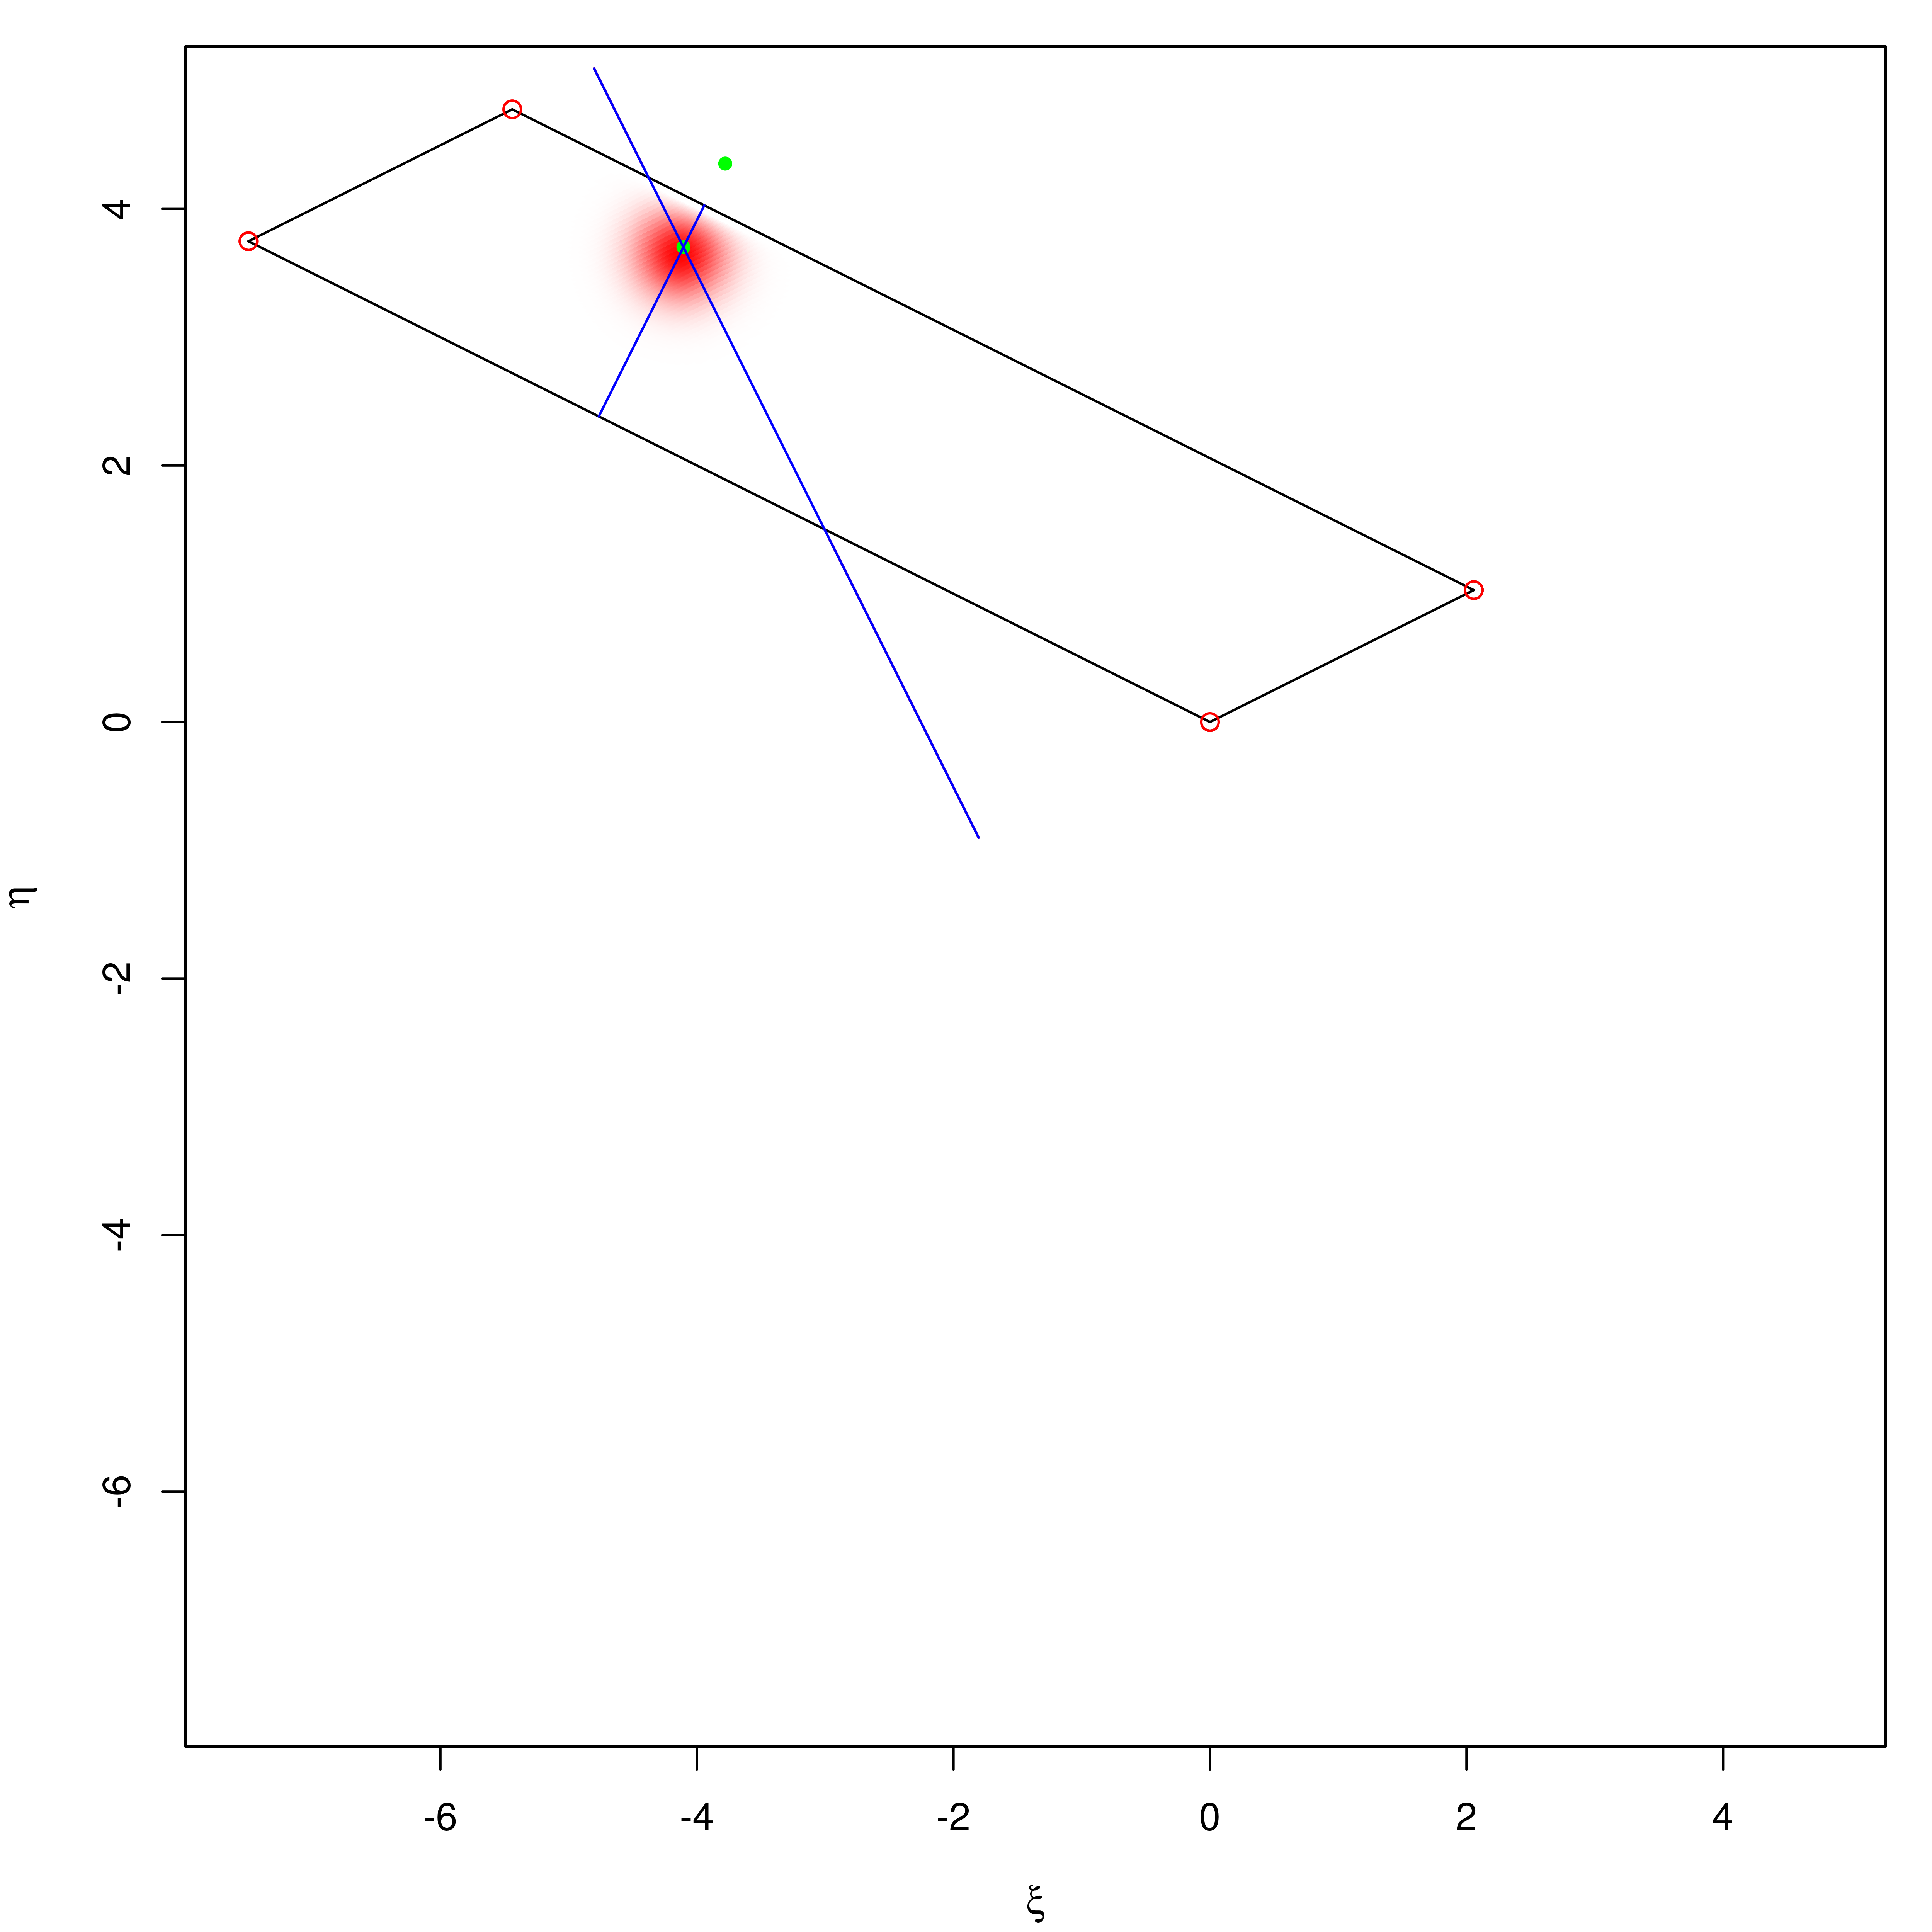
\includegraphics[width=1\linewidth]{../kernel-expansion/documentation/small-time-solution.png}
    \end{minipage}p
    %% 
    & \begin{minipage}{0.5\textwidth}
      \centering
      %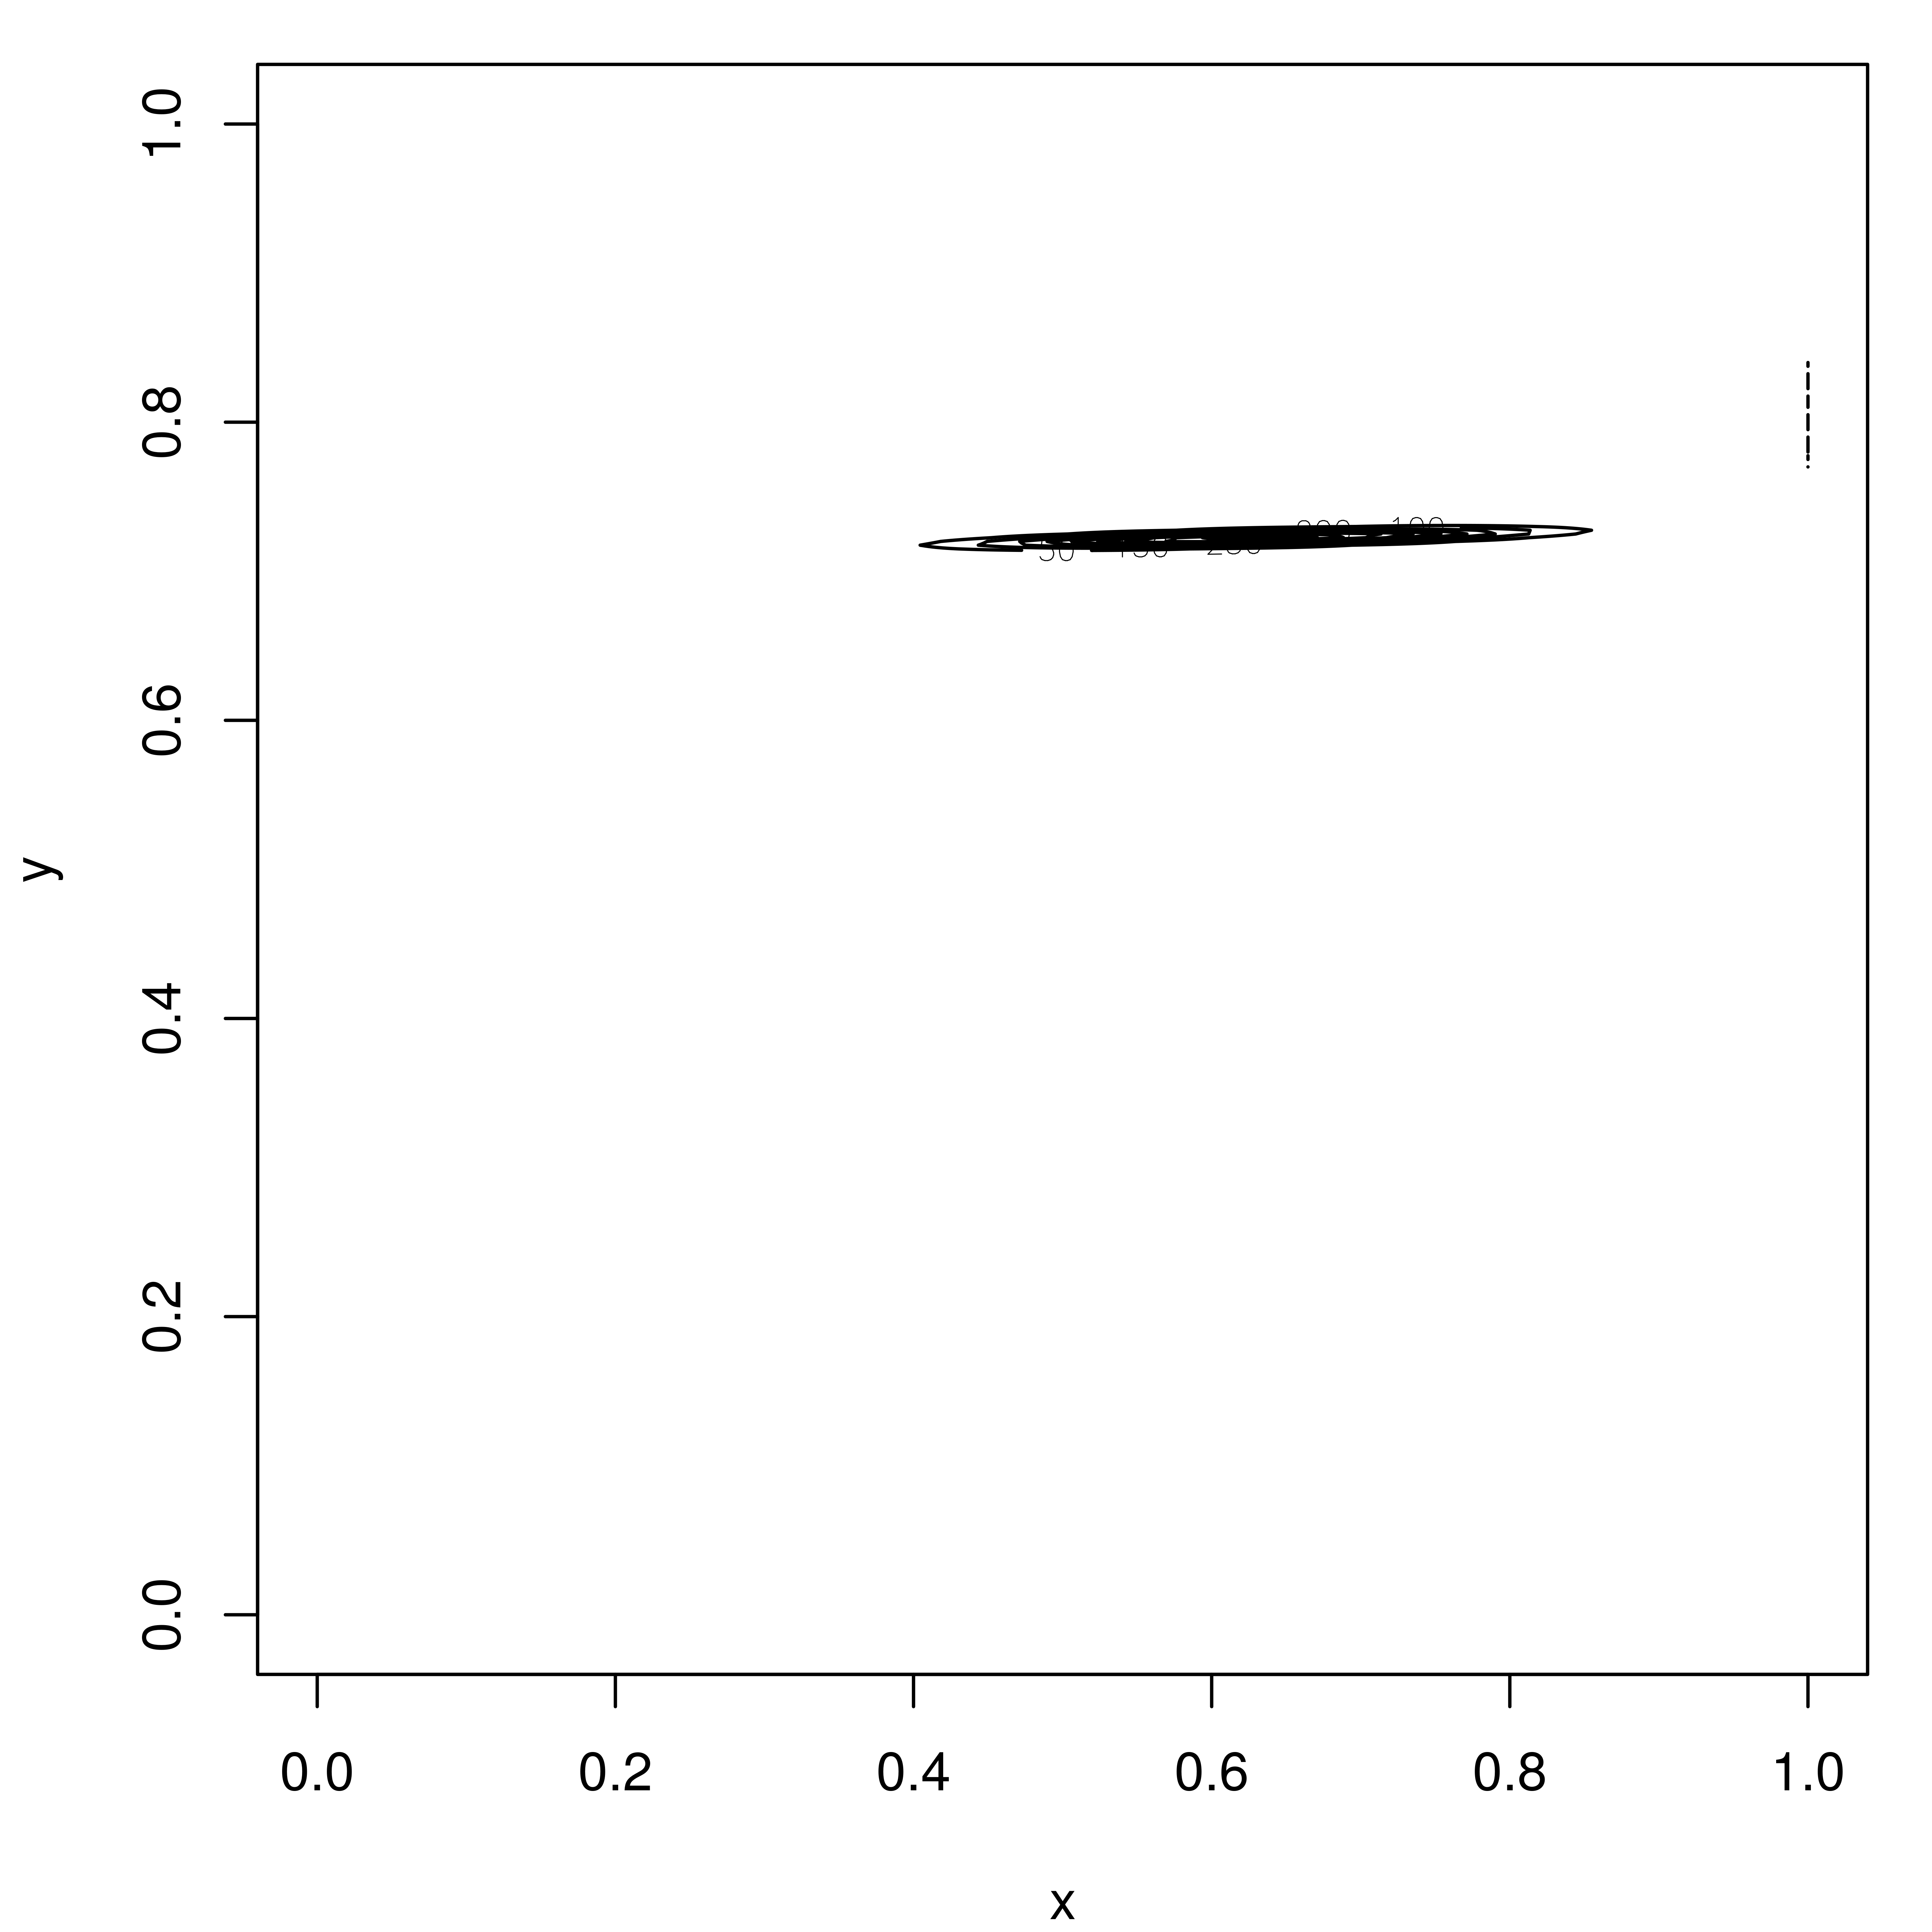
\includegraphics[width=1\linewidth]{../kernel-expansion/documentation/small-time-solution-contour.png}
    \end{minipage}
  \end{tabular}
  %%
  %%
  \caption{An example of the small-time solution
    $p(\xi,\eta,t_\epsilon)$ on the transformed domain
    $\tilde{\Omega}$ with $\tau_x = \tau_y = 1$ and $\rho=0.6$. Right:
    The shaded red region is a heatmap of the small-time solution in
    the transformed coordinate frame, while the blue line segments
    represent the distance between the boundaries and the initial
    condition coordinate. The green point outside of the computational
    domain is the center of the reflected image $(\xi_0', \eta_0')$
    about the closest boundary. Left: The small-time solution
    transformed back to the original coordinate system. Here, the
    contours denote the level-sets for the function. They very closely
    approximate the level sets for the fundamental solution of the
    unbounded problem (\ref{eq:qq})}
  \label{fig:step-1-small-time}
\end{figure}
Using Theorem 5.E of \cite{zeidler1995applied}, we can solve for
$p(x,y,t)$ by considering the smooth $p(x,y,t_\epsilon)$ as an initial
condition and evolving it forward in time by $t-t_\epsilon$. This
replaces initial condition orthogonality condition in
(\ref{eq:orthogonality-conditions-mat-2}) with
\begin{align}
  M \mathbf{c}(t_\epsilon) &= \mathbf{p}(t_\epsilon), \\
   [\mathbf{p}(t_\epsilon)]_i &= \displaystyle \int_\Omega p(x,y,t_\epsilon) \psi_i(x,y) dx\,dy. \nonumber
\end{align}
Intuitively, the bigger $t_\epsilon$, the smaller both $R_e(k)$ and
$R_0(k)$ will be, and the better our method will do.
% less eigenmodes present in $p(x,y,t_\epsilon)$, and the more accurate
% our weak solution according to the error estimate
% \[
%   \| e(t) \|_{L_2(\Omega)} \leq C h(k)^2 \| p(x,y,t_\epsilon) \|_{2}.
% \]


\subsection{Orthonormal Basis Family}
% An upper bound of the rate at which the Galerkin approximation
% converges to $p(x,y,t)$ is given by condition (\ref{eq:ic-bound}),
% namely by how well the initial condition may be approximated via a
% projection onto $S_k$.
We motivate the construction of the orthonormal basis functions by
once again considering the fundamental solution for the unbounded
problem (\ref{eq:qq}). In the absence of boundaries, (\ref{eq:qq}) is
solved by the function
\[
  G(x,y,t | x_0', y_0') = \frac{1}{2\pi\,\,t\,\, \tau_x\tau_y\sqrt{1-\rho^2}} \exp\left\{ -\frac{1}{2\,t(1-\rho^2)} \left( \frac{(x - x_0')^2}{\tau_x^2} - 2\rho \frac{(x-x_0')(y-y_0')}{\tau_x\tau_y} + \frac{(y - y_0')^2}{\tau_y^2}\right) \right\},
\]
with
$x_0' = (x_0 - a_x)/(b_x-a_x),\quad y_0' = (y_0 - a_y)/(b_y-a_y)$. We
choose the family of basis functions
$S_k = \left\{\psi_i(x,y), \,\, 0 \leq i \leq k \right\}$
\begin{align}
  \psi_i(x,y) &= \frac{1}{2\pi \sigma^2\sqrt{1-\tilde{\rho}^2} } \exp\left\{ -\frac{1}{2(1-\tilde{\rho}^2)\sigma^2} \left( (x - x_i)^2 - 2\tilde{\rho} (x-x_i)(y-y_i) + (y - y_i)^2 \right) \right\} x\left(1-x\right)\, y(1-y)
\end{align}
for some parameters $(\tilde{\rho}, \sigma)$ and a collection of nodes
$\{ (x_i,y_i) \}_{i=0}^k$ which form a grid over $\Omega$.

This grid is determined by the choice of kernel parameters
$(\tilde{\rho}, \sigma)$ with a scaling parameter $l$, and it is
defined in the following way. For $(\tilde{\rho}, \sigma, l)$, overlay
a grid $\{ (x'_j, y'_j) \}_{j=0}^{k'}$ such that
$(x'_0, y'_0) = (0.5,0.5)$ and the subsequent grid points are
$l\sigma(1 + \tilde{\rho})$ units apart in the $x-$direction and
$l\sigma(1 - \tilde{\rho})$ units apart in the $y-$direction over
$[1/2 - 1/\sqrt{2}, 1/2 + 1/\sqrt{2}] \, \times [1/2 - 1/\sqrt{2}, 1/2
+ 1/\sqrt{2}]$ (see left panel of Figure (\ref{fig:grids})).
%%
%%
\begin{figure}
  \centering
  %%
  %%
  \begin{tabular}{cc}
    \begin{minipage}{0.4\textwidth}
      \centering
      %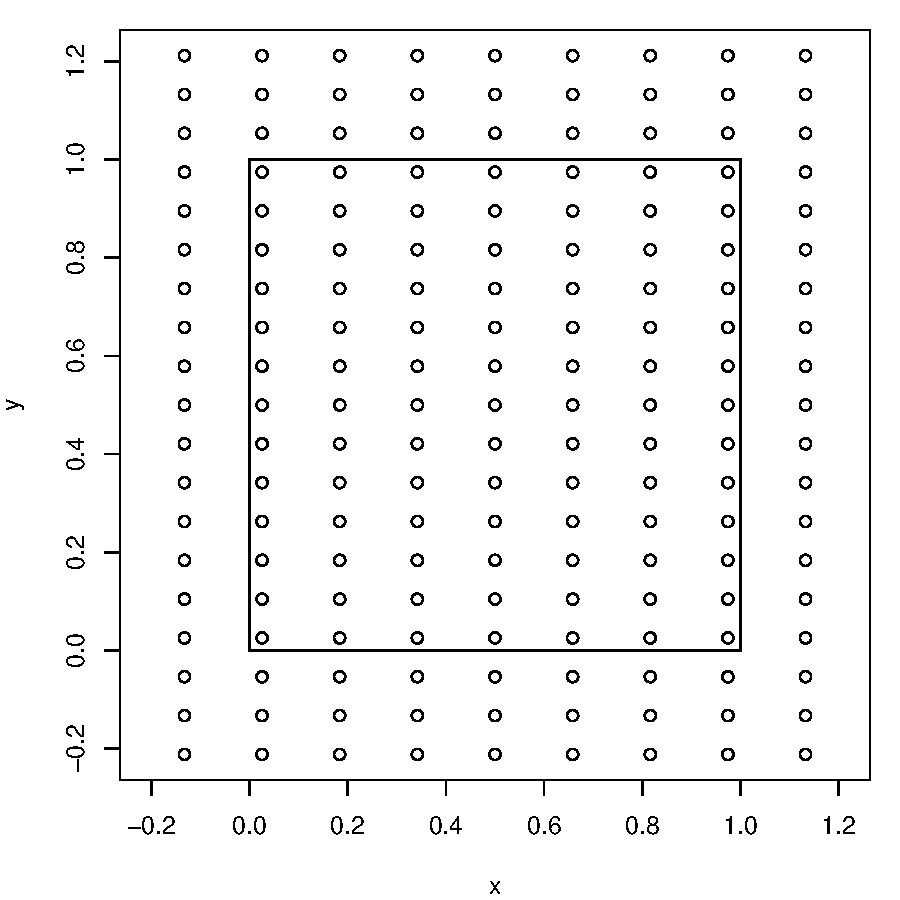
\includegraphics[width=1\linewidth]{../kernel-expansion/documentation/nodes-1.pdf}
    \end{minipage}
    %% 
    & \begin{minipage}{0.4\textwidth}
      \centering
      %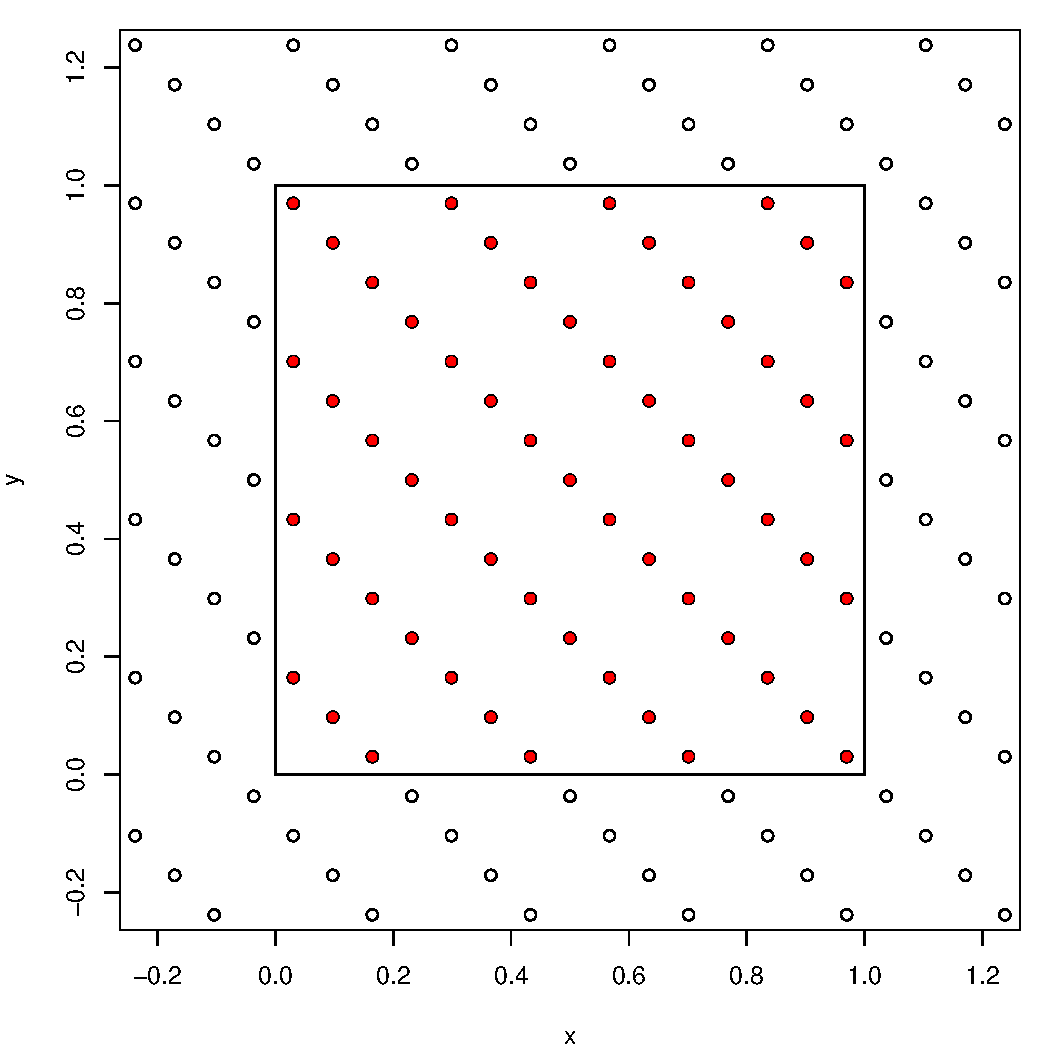
\includegraphics[width=1\linewidth]{../kernel-expansion/documentation/nodes-2.pdf}
    \end{minipage}
  \end{tabular}
  %%
  %%
  \caption{A sample grid design for $l=1$, $\sigma=0.3$ and $\rho=0.6$. The
    left panel corresponds to the initial grid
    $\{ (x'_j,y'_j) \}_{j=0}^{k'}$ over $\Omega$ (solid black
    square). The right panel depicts the rotated initial grid. The set
    of final node points $\{ (x_i,y_i) \}_{i=0}^{k}$ is contained
    within $\Omega$ and is denoted by the red solid points.}
  \label{fig:grids}
\end{figure}
%%
%%
Next, apply the clockwise, $\pi/4$ rotation centered on
$(1/2, 1/2)$ to each node
\begin{align*}
  \left( \begin{array}{c}
           x_j \\
           y_j
         \end{array} \right) =
       \left( \begin{array}{cc}
                1/\sqrt{2} & 1/\sqrt{2} \\
                -1/\sqrt{2} & 1/\sqrt{2}
              \end{array} \right) 
            \left( \begin{array}{c}
                     x'_j - 1/2\\
                     y'_j -1/2
                   \end{array} \right) +
  \left( \begin{array}{c}
           1/2 \\ 1/2
           \end{array} \right).
\end{align*}
The grid is comprised of all nodes within $\Omega$:
$\left\{(x_i, y_i)\right\}_{i=0}^k = \left\{ (x_j, y_j) | (x_j, y_j)
  \in \Omega, j = 0, \ldots, k' \right\}$ (see right panel of Figure
(\ref{fig:grids})). It should be noted that the level sets of the heat
kernel for the basis functions are ellipses with major and minor axes
aligned with the node points. Further, there is more resolution
(ie. the node layout is denser) along the direction corresponding to
the smaller standard deviation of the basis heat kernel in the
principal coordinate frame. Finally, for a given $l$, nodes in either
principal direction are separated by $l$ standard deviations of the
basis heat kernel. This layout naturally takes into account some
degree of correlation $\tilde{\rho}$ so that the small-time solution,
having level sets similar to those of the kernels, can be better
resolved. Essentially, the collection
$\{ \psi_i(x,y| \tilde{\rho}, \sigma) \}_{i=0}^k$ is composed of
fundamental solutions to a heat diffusion problem tuned by $\sigma$
and $\tilde{\rho}$, tampered such that their support is on $\Omega$,
zero on the boundaries, still smooth, and inheriting the correlation
structure of the fundamental solution to the problem. More basis
elements are added by decreasing $\sigma$ and altering $l$, while the
degree of correlation is controlled by $\tilde{\rho}$. For
the purposes of this paper, we found that keeping fixed $l=1$ with a
moderate $\tilde{\rho}$ ($|\tilde{\rho}| \sim 0.6$) yields reasonable
results. It is important, however, that
$\mbox{sign}(\tilde{\rho}) = \mbox{sign}(\rho)$ so that the
problematic, narrow component of the small-time solution (which can be
seen in the minor axis of the contours of the small-time solution in
the right panel of Figure (\ref{fig:step-1-small-time})) can be
resolved.

%
%In this manner,
% our basis function choice is in keeping with the golden rule for the
% rate of convergence: \textbf{The smoother the solution to the original
%   problem and the smoother the functions in the basis space, the
%   faster the convergence of the Ritz-Galerkin method.} (Remark 1(c) in
%   Chapter 2 of \cite{zeidler1995applied}).

At this point, having explicitly defined
$\psi_i(x,y|\sigma,\tilde{\rho})$, it should be noted that these basis
functions are constant with respect to the normalized problem
parameters $(\tau_x, \tau_y, \rho)$. Thus, the derivative of Galerkin
approximation $p^{(k)}$ with respect to the boundaries takes on the
form
\[
  \frac{\partial^4}{\partial a_x \partial b_x \partial a_y \partial
    b_y} p^{(k)}(x,y,t) = \boldsymbol{\psi}(x,y)^T
  \frac{\partial^4}{\partial a_x \partial b_x \partial a_y \partial
    b_y} \left\{ \exp\left( M^{-1}S\, t \right) \mathbf{c}(0) \right\},
\]
which is well-defined given the discussion above.

\subsection{Error Bound} \label{sec:error-bound}
A bound on the closeness of the approximate solution $p^{(k)}(x,y,t)$
to the strong solution $p(x,y,t)$ is developed in
\cite{bramble1977some}.  Their result shows that the Galerkin
approximation we use converges to the strong solution in
$L_2(\Omega)$, and it motivates the thrust of our numerical
solution. First, we define the \textit{error} term
\[
  e^{(k)}(t) = p(x,y,t) - p^{(k)}(x,y,t),
\]
as well as the norm
\[
  \| w \|_2 = \sum_{j=0}^\infty \lambda_j^2 \left<w, \phi_j\right>^2
\]
for the eigenpairs $(\lambda_j, \phi_j)$ of the operator
$\mathcal{L}$. As referred to in \cite{bramble1977some}, functions
$w \in L_2(\Omega)$ with $\|w\|_2 < \infty$ are also in
$W_2^2(\Omega)$. Finally, if we have the condition (corresponding to
equation 2.1 in \cite{bramble1977some})
\begin{align}
  \| p(x,y,t_\epsilon) - p^{(k)}(x,y,t_\epsilon) \|_{L_2(\Omega)} &\leq C\, h(k)^2 \| p(x,y,t_\epsilon) \|_2, \label{eq:ic-bound}
\end{align}
where $h(\cdot)$ is a decreasing function of $k > 0$, Theorem 2.1 in
\cite{bramble1977some} applies and we have the error estimate
\begin{align}
  \| e^{(k)}(t) \|_{L_2(\Omega)} \leq C h(k)^2 \| p(x,y,t_\epsilon) \|_{2}. \label{eq:error-est}
\end{align}
Here, the  constant $C$  and the  function $h(k)$ are  the same  as in
(\ref{eq:ic-bound}). The implication is that if the basis functions in
$S_k$ represent  the small-time  solution $p(x,y,t_\epsilon)$  with no
error, the Galerkin solution forward in time is also without error.

We can ensure condition (\ref{eq:ic-bound}) is met if $S_k$ is
complete in $L_2(\Omega)$ as $k$ grows. The other two conditions
necessary for the error bound to apply are demonstrated by
\cite{bramble1977some} for the Galerkin method. Equation
(\ref{eq:error-est}) can be summarized in a simple way: the
\textit{error} of the method is controlled by how much variation the
small-time solution has; the \textit{rate} of decrease of the error is
controlled by how well the span of $S_k$ represents the small-time
solution compared to the variation of the initial condition as $k$
increases. In the context of (\ref{eq:error-est}), our method, with
its small-time analytic solution and choice of basis functions, is
specifically tailored to minimize the error between the strong
solution and its Galerkin approximation under $L_2(\Omega)$.

% However, the initial condition for (\ref{eq:qq}) requires all in
% eigenmodes being included in the representation of the initial
% conditions, so that
% \[
%   \| p(x,y,0) \|_{2} = \left\| \delta\left( x - \frac{x_0 - a_x}{b_x-a_x}
%   \right) \delta\left( y - \frac{y_0 - a_y}{b_y-a_y} \right)\right\|_{2} = +\infty.
% \]
% It is obvious that we cannot apply the error estimates above. However,
% evolving the solution forward in time, even for a short period,
% diffuses the delta-function IC and attenuates out the highest
% frequency modes. Further, because solutions to the diffusion equation
% are smooth, $p(x,y,t_\epsilon)$ will give us a smooth initial function
% which will make the error bounds admissible.


\section{Estimation}
Consider the problem of estimating the parameters
$(\mu_x, \mu_y, \sigma_x, \sigma_y, \rho)$ from an i.i.d. set of
samples $(Z_1, \ldots, Z_n)$ from random variable $Z(t)$ at a given
value of $t$ in the process in (1)-(2). Specifically, $Z(t)$ is formed
as
$$ Z(t) =( X(t), Y(t), m_x(t), M_x(t), m_y(t), M_y(t)) $$
where 
$$m_x(t)= \min_{0 \le t' \le t} X(t), \;\; 
M_x(t)= \max_{0 \le t' \le t} X(t), \;\; m_y(t)= \min_{0 \le t' \le t}
Y(t), \;\; M_y(t)= \max_{0 \le t' \le t} Y(t). $$ We say that $Z_i$ is
sampled from the distribution corresponding to the probability density
function (\ref{eq:pdf})
\[
  Z_i \sim F(\theta),
\]
where the cumulative distribution function $F$ has the usual interpretation
\begin{align*}
  F(z = (x, y, a_x, b_x, a_y, b_y) | \theta) &= \Pr\left(X(t) \leq x,
    Y(t) \leq y, m_x \leq a_x, M_x \leq b_x, m_y \leq a_y, M_y \leq b_y\right).
\end{align*}

This estimation problem is of particular importance in quantitative
finance where the model equations (\ref{eq:X}) - (\ref{eq:Y}) (with
various bells and whistles attached) are widely used. However, to the
best of our knowledge, all current \textit{likelihood} methods in the
literature either ignore the observed maximum/minimum information or
use only some of it. Likelihood-free approaches, like that of
\cite{rogers1991estimating}, on the other hand suffer from not being
able to be easily integrated into inferential frameworks that require
explicit estimates of probability.

Since we do not have a closed-form solution for the likelihood, we
will use an iterative derivative-free maximization algorithm (the
Nelder-Mead method; see \cite{lagarias1998convergence} for review and
convergence properties) which requires repeated evauluation of the
likelihood. For moderate to large samples sizes this is feasible,
because our numerical method is specifically designed for
computational efficiency for repeatedly evaluating the density
function (\ref{eq:pdf}). The maximum likelihood estimator (MLE) for
the true parameters based on $n$ samples, which we call
$\hat{\theta}_n := (\hat{\mu}_x, \hat{\mu}_y, \hat{\sigma}_x,
\hat{\sigma}_y, \hat{\rho})$, is especially useful in practical
settings when it exhibits \textit{consistency}, \textit{i.e.}: the MLE
gets closer to the true parameter vector $\theta$ as more data is
collected and included in the likelihood (assuming the model and its
parameters remain constant during the data collection). More
precisely, the estimator $\hat{\theta}_n$ is consistent if it
converges in probability to the true parameter:
\[
  \Pr( | \hat{\theta}_n - \theta | ) \to 0 \qquad \mbox{as} \qquad n \to \infty.
\]

\subsection{Consistency}
In this section we prove that the MLE based on the Galerkin
approximation $p^{(k)}(x,y,t)$ to the governing Fokker-Planck equation
(\ref{eq:1}) is consistent. To do so, we first show that the
distribution on $Z$ based on the approximate $p^{(k)}(x,y,t)$ converges to
the true distribution $F(\cdot | \theta)$. Define the probability densities
\begin{align}
  f(z) &= f(x,y,a_x,b_x,a_y,b_y) := \Pr\left(X(t) \in dx, Y(t) \in dy, m_x \in da_x,
         M_x \in db_x, m_y \in da_y, M_y \in db_y \left| \theta \right.\right) \label{eq:stong-density} \\
    f^{(k)}(z) &= f^{(k)}(x,y,a_x,b_x,a_y,b_y) := \frac{\partial^4}{\partial a_x \partial b_x \partial a_y \partial
         b_y} q^{(k)}(x,y,t | a_x, b_x, a_y, b_y). \label{eq:galerkin-density}
\end{align}
The function $f(z)$ is the probability density function corresponding
to $q(x,y,t)$, the strong solution to the governing Fokker-Planck
equation; $f^{(k)}(z)$ corresponds to the approximate solution
$q^{(k)}$ of the unnormalized equation obtained from the Galerkin
approximation $p^{(k)}$ of the normalized equation. Before proceeding,
we should note that both $f(z)$ and $f^{(k)}(z)$ exist. So see the
case for $f(z)$, consider the relation
\begin{align*}
  &f(x,y,a_x,b_x,a_y,b_y) = \\
  &\Pr\left(X(t) \in dx, Y(t) \in dy, m_x \in da_x, M_x \in db_x, m_y
  \in a_y, M_y \in db_y \left| \theta \right.\right) = \\
  &\mathbb{P}_{W}\left( \underbrace{\left\{ \omega \in W \left| X_\omega(t) = x,
  Y_\omega(t)=y, \inf_{t'\in [0,1]} X_\omega(t') = a_x,
  \sup_{t'\in [0,1]} X_\omega(t') = b_x, \inf_{t'\in [0,1]}
        Y_\omega(t') = a_y, \sup_{t'\in [0,1]} Y_\omega(t') = b_y
      \right. \right\}}_{A(x,y,a_x,b_x,a_y,b_y) = A(z)}\right)
\end{align*}
where $\mathbb{P}_{W}$ is the Wiener measure on the sample space $W$
of all realizations (paths) $(X_\omega(t), Y_\omega(t))$ from the
stochastic process (\ref{eq:X}) - (\ref{eq:Y}) defined in the usal way
using Kolmogorov's extension of measure over cylinder sets on
$t \to \mathbb{R}^2$ (see \cite{freidlin1985functional}, Section
1.2). Sets of the form $A(x,y,a_x,b_x,a_y,b_y)$ can be defined as a
countable intersection/union of cyliner sets on $t \to \mathbb{R}^2$,
hence they are measurable under $\mathbb{P}_{W}$; therefore $f(z)$ exists and
is bounded above by 1. Moreover, since $q(x,y,t|a_x,b_x,a_y,b_y)$ represents the
integral of $f(z)$ with respect to the boundary variables, we have
\[
  f(x,y,a_x,b_x,a_y,b_y) = \frac{\partial^4}{\partial a_x \partial b_x \partial a_y \partial
         b_y} q(x,y,t | a_x, b_x, a_y, b_y).
\]
The existence of $f^{(k)}(z)$ as defined in
(\ref{eq:galerkin-density}) is guaranteed by Theorem 4.1 in
\cite{singler2008differentiability}. The result states that weak
solutions to parabolic problems are differentiable with respect to
parameters as long as the weak (Galerkin-form) operator
$\left< \mathcal{L} \psi_i(x,y), \psi_j(x,y) \right>$ is
differentiable with respect to the parameters. The condition certainly
holds for the normalized problem (\ref{eq:qq}) with our choice of
basis functions $S_k$, as they are infinitely differentiable with
repsect to $x,y$, the boundaries, and the diffusion parameters. 

At this point we will assume that for a sufficiently large $k$,
$f^{(k)}(z)$ is positivie for all $z \in Z$ and is integrable over
$Z$. As such, we may regard it as a proper probability density
function with the cumulative probability density and probability
measure over $Z$ being 
\begin{align}
  F^{(k)}(z | \theta) &= \displaystyle \int_{-\infty}^{a_x} \displaystyle \int_{-\infty}^{a_y} \displaystyle \int_{-\infty}^{b_x} \displaystyle \int_{-\infty}^{b_y} \displaystyle \int_{-\infty}^x \displaystyle \int_{-\infty}^y \frac{\partial^4}{\partial a'_x \partial b'_x \partial a'_y \partial b'_y} q^{(k)}(x', y', t | a'_x, b'_x, a'_y, b'_y)\,\,\, dx'\, dy'\, da'_x\, db'_x\, da'_y\, db'_y, \label{eq:approx-measure} \\
                          \Pr_{k}(A) &:= \displaystyle \int_{A} f^{(k)}(z)\, dz, \quad \mbox{ for any measurable } A \subset Z. \label{eq:approx-measure-2}
\end{align}
We will prove that for every $z \in Z$,
\[
  \lim_{k\to \infty} F^{(k)}(z | \theta) = F(z | \theta).
\]
First, we prove the Lemma
\begin{lemma}\label{lem:1}
  For $z = (x, y, a_x, b_x, a_y, b_y)$,
  \[
    \lim_{k\to \infty} \displaystyle \int_{a_x}^{b_x} \displaystyle
    \int_{a_y}^{b_y} f^{(k)}(x,y,a_x,b_x,a_y,b_y)\, dx\,dy =
    \displaystyle \int_{a_x}^{b_x} \displaystyle \int_{a_y}^{b_y}
    f(x,y,a_x,b_x,a_y,b_y)\, dx\,dy.
  \]
\end{lemma}
\begin{proof}
  Define the sets of form, for $z = (x,y,a_x,b_x,a_y,b_y)$,
  \begin{align*}
    B(a_x, b_x, a_y, b_y) &= \left\{ z' \in Z \left| z' \in [a_x, b_x]
        \times [a_y, b_y] \times [a_x, \infty) \times (-\infty, b_x]
                            \times [a_y, \infty) \times (-\infty, b_y] \right.\right\}.
  \end{align*}
  Elements within $B(a_x, b_x, a_y, b_y)$ are equivalent to sample paths that stay within the region $[a_x, b_x] \times [a_y, b_y]$:
  \begin{align*}
    B(a_x, b_x, a_y, b_y) &= \left\{ \omega \in W | X_\omega(t) \in [a_x, b_x], Y_\omega(t) \in [a_y, b_y], m_x \in [a_x,b_x), M_x \in (a_x, b_x] \right\}
  \end{align*}

  Then
  \begin{align}
    \Pr(B(a_x, b_x, a_y, b_y)) &= \displaystyle \int_{B(a_x, b_x, a_y, b_y)} f(z)\, dz \nonumber \\ 
                               &= \displaystyle \int_{a_x}^{\infty} \displaystyle \int_{-\infty}^{b_x} \displaystyle \int_{a_y}^{\infty} \displaystyle \int_{-\infty}^{b_y} \displaystyle \int_{-\infty}^{b_x} \displaystyle \int_{-\infty}^{b_y} f(x', y', a'_x, b'_x, a'_y, b'_y) dx' dy' da_x' db_x' da_y' db_y' \label{eq:full-form} \\
                               &= \displaystyle \int_{a_x}^{b_x} \displaystyle \int_{a_y}^{b_y} q(x,y,a_x,b_x,a_y,b_y)\, dx\, dy, \nonumber
  \end{align}
  
  where the last equality employs the interpretation of $q$ in
  (\ref{eq:CDF}) and we can freely change the order of integration as
  $f$ is bounded for all $z \in Z$. Similarly,
  \begin{align*}
    \Pr_k(B(a_x, b_x, a_y, b_y)) &= \displaystyle \int_{a_x}^{b_x} \displaystyle \int_{a_y}^{b_y} q^{(k)}(x,y,a_x,b_x,a_y,b_y)\, dx\, dy.
  \end{align*}
  From (\ref{eq:full-form}), the partial derivative of the probability
  $\Pr(B(a_x,b_x,a_y,b_y))$ is well-defined and can be written as
  \begin{align*}
    \frac{\partial^4}{\partial a_x \partial b_x \partial a_y \partial b_y} \Pr(B(a_x, b_x, a_y, b_y)) &= \displaystyle \int_{a_x}^{b_x} \displaystyle \int_{a_y}^{b_y} f(x,y,a_x,b_x,a_y,b_y)\, dx\, dy.
  \end{align*}
  The second-order \textbf{finite difference} approximation the above
  expression can be expressed as a linear combination of probabilities
  of perturbed sets $B(\cdot)$:
  \begin{align*}
    \lim_{\epsilon \to 0}\quad \frac{1}{\epsilon^4} \sum_{i=1}^{16} c(i) \Pr(B(a_x + k_1(i)\epsilon, b_x + k_2(i)\epsilon, a_y + k_3(i)\epsilon, b_y + k_4(i)\epsilon) = \frac{\partial^4}{\partial a_x \partial b_x \partial a_y \partial b_y} \Pr(B(a_x, b_x, a_y, b_y)),
  \end{align*}
  where $c$ and $k$ are functions from $i$ to the appropriate
  coefficients in the second-order finite difference approximation
  $c(i) \to \left\{-1, 1\right\}$, $k_j(i) \to \{-1,1\}$. Using Big-O
  notation, for a sufficiently small $\epsilon$
  \begin{equation}
    \sum_{i=1}^{16} c(i) \Pr(B(a_x + k_1(i)\epsilon, b_x +
    k_2(i)\epsilon, a_y + k_3(i)\epsilon, b_y + k_4(i)\epsilon) =
    \epsilon^4 \frac{\partial^4}{\partial a_x \partial b_x \partial
      a_y \partial b_y} \Pr(B(a_x, b_x, a_y, b_y)) + O(\epsilon^6 ;
    a_x, b_x, a_y, b_y). \label{eq:fin-diff}
  \end{equation}

  The convergence result in Section \ref{sec:error-bound} implies that
  \begin{align*}
    \Pr_k(B(a_x + k_1(i)\epsilon, b_x + k_2(i)\epsilon, a_y +
    k_3(i)\epsilon, b_y + k_4(i)\epsilon) = \displaystyle \int_{a_x +
    k_1(i)\epsilon}^{b_x + k_2(i)\epsilon} \displaystyle \int_{a_y + k_3(i)\epsilon}^{b_y +
    k_4(i)\epsilon} q^{(k)}(x,y,a_x,b_x,a_y,b_y)\, dx\, dy \to \\
    \displaystyle
    \int_{a_x + k_1(i)\epsilon}^{b_x + k_2(i)\epsilon} \displaystyle \int_{a_y +
    k_3(i)\epsilon}^{b_y + k_4(i)\epsilon} q(x,y,a_x,b_x,a_y,b_y)\, dx\, dy =
    \Pr(B(a_x + k_1(i)\epsilon, b_x + k_2(i)\epsilon, a_y +
    k_3(i)\epsilon, b_y + k_4(i)\epsilon) \\
    \mbox{ as } k \to \infty \mbox{ in } L_2(\Omega).
  \end{align*}
  Hence, for a sufficiently large $k$ dependent on the supremum over
  $i$, and given the error estimate in (\ref{eq:error-est}), we have
  the relation
  \begin{align*}
    \Pr_k(B(a_x + k_1(i)\epsilon, b_x + k_2(i)\epsilon, a_y +
    k_3(i)\epsilon, b_y + k_4(i)\epsilon) &= \Pr(B(a_x + k_1(i)\epsilon, b_x + k_2(i)\epsilon, a_y +
                                            k_3(i)\epsilon, b_y + k_4(i)\epsilon) \\
    & + O(h(k)^2; a_x + k_1(i)\epsilon, b_x + k_2(i)\epsilon, a_y + k_3(i)\epsilon, b_y + k_4(i)\epsilon)
  \end{align*}
  Note here that the dominating terms $O(h(k)^2; \cdot)$ are
  differentiable with respect to the boundary parameters
  $(a_x, b_x, a_y, b_y)$ since $q$ and $q^{(k)}$ have this
  property. Therefore, if we replace $\Pr(\cdot)$ in
  (\ref{eq:fin-diff}) with $\Pr_k(\cdot)$
  \begin{align*}
    \sum_{i=1}^{16} c(i) \Pr_k(B(a_x + k_1(i)\epsilon, b_x +
    k_2(i)\epsilon, a_y + k_3(i)\epsilon, b_y + k_4(i)\epsilon) &= \sum_{i=1}^{16} c(i) \Pr(B(a_x + k_1(i)\epsilon, b_x +
                                                                  k_2(i)\epsilon, a_y + k_3(i)\epsilon, b_y + k_4(i)\epsilon)  \\
                                                                & + \sum_{i=1}^{16} c(i) O(h(k)^2; a_x + k_1(i)\epsilon, b_x +
                                                                  k_2(i)\epsilon, a_y + k_3(i)\epsilon, b_y + k_4(i)\epsilon) \\
    &=     \epsilon^4 \frac{\partial^4}{\partial a_x \partial b_x \partial
      a_y \partial b_y} \Pr(B(a_x, b_x, a_y, b_y)) + O(\epsilon^6 ;
      a_x, b_x, a_y, b_y) \\
                                                                & + \sum_{i=1}^{16} c(i) O(h(k)^2; a_x + k_1(i)\epsilon, b_x +
                                                                  k_2(i)\epsilon, a_y + k_3(i)\epsilon, b_y + k_4(i)\epsilon).
  \end{align*}
  Dividing both sides by $\epsilon^4$ produces
  \begin{align*}
    \frac{1}{\epsilon^4} \sum_{i=1}^{16} c(i) \Pr_k(B(a_x + k_1(i)\epsilon, b_x +
    k_2(i)\epsilon, a_y + k_3(i)\epsilon, b_y + k_4(i)\epsilon) &= \frac{\partial^4}{\partial a_x \partial b_x \partial
                                                                  a_y \partial b_y} \Pr(B(a_x, b_x, a_y, b_y)) + O(\epsilon^2;
                                                                  a_x, b_x, a_y, b_y) \\
                                                                &+ \frac{1}{\epsilon^4}\sum_{i=1}^{16} c(i) O(h(k)^2; a_x + k_1(i)\epsilon, b_x +
                                                                  k_2(i)\epsilon, a_y + k_3(i)\epsilon, b_y + k_4(i)\epsilon) \\
    % = \frac{\partial^4}{\partial a_x \partial b_x \partial
    % a_y \partial b_y} \Pr(B(a_x, b_x, a_y, b_y)) + O(\epsilon;
    % a_x, b_x, a_y, b_y) + \frac{\partial^4}{\partial a_x \partial b_x \partial
    % a_y \partial b_y} O(h(k)^2 ; a_x, b_x, a_y, b_y)
  \end{align*}
  As mentioned above $O(h(k)^2; \cdot)$ is differentiable with respect
  to the boundary parameters, so that the right-most term is still
  $O(h(k)^2)$ as $\epsilon \to 0$. Taking the limit in $\epsilon$, we have
  \begin{align*}
    \displaystyle \int_{a_x}^{b_x} \displaystyle \int_{a_y}^{b_y}
    f^{(k)}(x,y,a_x,b_x,a_y,b_y)\, dx\, dy =
    \frac{\partial^4}{\partial a_x \partial b_x \partial a_y \partial
    b_y} \Pr_k(B(a_x, b_x, a_y, b_y)) \\
    = \frac{\partial^4}{\partial
      a_x \partial b_x \partial a_y \partial b_y} \Pr(B(a_x, b_x, a_y,
    b_y)) +  O(h(k)^2; a_x, b_x, a_y, b_y) \\
    =\displaystyle \int_{a_x}^{b_x} \displaystyle \int_{a_y}^{b_y}
    f(x,y,a_x,b_x,a_y,b_y)\, dx\, dy + O(h(k)^2; a_x, b_x, a_y, b_y).
  \end{align*}
  Therefore, we have the desired result:
  \[
    \lim_{k\to \infty} \displaystyle \int_{a_x}^{b_x} \displaystyle
    \int_{a_y}^{b_y} f^{(k)}(x,y,a_x,b_x,a_y,b_y)\, dx\,dy =
    \displaystyle \int_{a_x}^{b_x} \displaystyle \int_{a_y}^{b_y}
    f(x,y,a_x,b_x,a_y,b_y)\, dx\,dy.
  \]
\end{proof}

\begin{lemma}[Convergence in distribution] \label{lem:conv-dist}
  For any $z \in Z$,
  $ \lim_{k \to \infty} F^{(k)}(z | \theta) = F(z).$

\end{lemma}

\begin{proof}
  Let
  $I^{(k)}(z) = \displaystyle \int_{a_x}^{x} \displaystyle
  \int_{a_y}^{y} f^{(k)}(u,v,a_x,b_x,a_y,b_y)\, du\,dv$ and let
  $I(z) = \displaystyle \int_{a_x}^{x} \displaystyle \int_{a_y}^{y}
  f(u,v,a_x,b_x,a_y,b_y)\, du\,dv$. It is possible to show that
  $\lim_{k\to \infty} I^{(k)}(z) = I(z)$ as a consequence of Lemma
  \ref{lem:1} by considering some $\chi_k(z) \in S_k$ approximating
  the indicator $1(u \leq x, v \leq y)$ as $k \to \infty$ and setting up a triangle
  inequality. However, we will omit this technical detail here.

  Next, we know that $I(z)$ is integrable over $(a_x, b_x, a_y, b_y)$
  as $\Pr(Z) = \mathbb{P}_{W}(W) = 1$. The Dominated Convergence
  Theorem applies, and we therefore have
  \[
    \lim_{k \to \infty} \displaystyle \int_{-\infty}^{a_x} \displaystyle \int_{-\infty}^{b_x} \displaystyle \int_{-\infty}^{a_y} \displaystyle \int_{-\infty}^{b_y} I^{(k)}(z) da_x' db_x' da_y' db_y' = \displaystyle \int_{-\infty}^{a_x} \displaystyle \int_{-\infty}^{b_x} \displaystyle \int_{-\infty}^{a_y} \displaystyle \int_{-\infty}^{b_y} I(z) da_x' db_x' da_y' db_y',
  \]
  which implies the result of the Lemma.
\end{proof}
% \begin{align*}
%   q(x,y,t) = \\
%   \Pr\left(X(t) \in dx, Y(t) \in dy,  \min_{t'}X(t') \geq a_x,
%   \max_{t'}X(t')\leq b_x, \min_{t'} Y(t')\geq a_y, \max_{t'} Y(t')\leq b_y|  X(0)=x_0, Y(0)=y_0, \theta \right) = \\
%   \Pr_{W}\left(\left\{ \omega \in \Omega | X_\omega(t) \in dx,\,\, Y_\omega(t) \in dy,\,\,  \forall t' \in [0,t]\,\, a_x \leq X_\omega(t') \leq b_x,\,\, \forall t' \in [0,t] \,\, a_b \leq Y_\omega(t') \leq b_y,\,\, X_\omega(0) = Y_\omega(0) = 0 \right\} \right)
% \end{align*}
% Our strategy will be to define a family of sets $\left\{ \tilde{A}_m(z) \right\}_{m=0}^\infty$ for any $z=(x,y,a_x,b_x,a_y,b_y)$ such that
% \begin{align*}
%   \lim_{m \to \infty} \Pr_W \left(  \tilde{A}_m(z) \right) = 
%   \Pr \left( X(t) \leq x,
%   Y(t) \leq y, \min_{t' \leq t} X(t') \leq a_x, \max_{t' \leq t}
%   X(t') \leq b_x, \min_{t' \leq t} Y(t') \leq a_y, \max_{t' \leq t}
%   Y(t') \leq b_y \right) = F(z | \theta)
% \end{align*}

% \begin{lemma}
%   For $z = (x,y,a_x,b_x,a_y,b_y)$, 
%   \[\lim_{m \to \infty} \displaystyle \int_{-\infty}^x \displaystyle
%     \int_{-\infty}^y q(x',y',t, a_x-m, b_x, a_y-m, b_y)\,\, dx'\,dy' -
%     \displaystyle \int_{-\infty}^x \displaystyle \int_{-\infty}^y
%     q(x',y',t, a_x, b_x, a_y, b_y)\,\, dx'\,dy' = F(z | \theta)\]
% \end{lemma}
% \begin{proof}
% Given some $z = (x,y,a_x,b_x,a_y,b_y)$, define the sets
% \begin{align*}
%   A_m(z) &= \left\{ \omega \in \Omega | X_\omega(t) \leq x,\,\,
% Y_\omega(t) \leq y,\,\, \right. \\ & \forall t' \in [0,t]\,\, a_x-m
% \leq X_\omega(t') \leq b_x,\,\, \\ & \forall t' \in [0,t] \,\, a_y -
% m\leq Y_\omega(t') \leq b_y,\,\, \\ & \left.X_\omega(0) = Y_\omega(0)
% = 0 \right\}, \quad \quad m = 0,1,2,... \\
% \end{align*}
% Note here that $\Pr_{W}(A_m(z)) = \displaystyle \int_{-\infty}^x \displaystyle \int_{-\infty}^y q(x',y',t, a_x-m, b_x, a_y-m, b_y)\,\, dx'\,dy'$.  Next, we define
% \begin{align*}
%   \tilde{A}_{m}(z) &= A_m(z) \,\, \bigcap \,\, A_0^C(z) \\
%                    &= \left\{ \omega \in \Omega | X_\omega(t) \in dx,\,\, \right.\\
%                    & \quad \quad \forall t' \in [0,t]\,\, a_x-m \leq X_\omega(t') \leq b_x,\,\, \\
%                    & \quad \quad \forall t' \in [0,t] \,\, a_y - m\leq Y_\omega(t') \leq b_y,\,\, \\
%                    & \quad \quad \exists t_{a_x} \in [0,t] \,\, s.t. \,\, X_\omega(t_{a_x}) < a_x \,\, , \exists t_{a_y} \in [0,t] \,\, s.t. \,\, X_\omega(t_{a_y}) < a_y, \\
%                    & \quad \quad \left.X_\omega(0) = Y_\omega(0) = 0 \right\}
% \end{align*}
% It is easy to see that $A_{m}(z) \subset A_{m+1}(z)$ and that
% $\tilde{A}_{m}(z) \subset \tilde{A}_{m+1}(z)$. Because of the former
% relation,
% \[
%   \Pr_{W}(\tilde{A}_m(z)) = \Pr_W(A_m(z)) - \Pr_{W}(A_0(z)) = \displaystyle \int_{-\infty}^x \displaystyle \int_{-\infty}^y q(x',y',t, a_x-m, b_x, a_y-m, b_y)\,\, dx'\,dy' - \displaystyle \int_{-\infty}^x \displaystyle \int_{-\infty}^y q(x',y',t, a_x, b_x, a_y, b_y)\,\, dx'\,dy'.
% \]
% Finally,
% \begin{align*}
%   \bigcup_{m=0}^\infty \tilde{A}_m(z) &= \left\{ \omega \in \Omega | X_\omega(t) \in dx,\,\, \right.\\
%                    & \quad \quad \forall t' \in [0,t]\,\, -\infty \leq X_\omega(t') \leq b_x,\,\, \\
%                    & \quad \quad \forall t' \in [0,t] \,\, -\infty \leq Y_\omega(t') \leq b_y,\,\, \\
%                    & \quad \quad \exists t_{a_x} \in [0,t] \,\, s.t. \,\, X_\omega(t_{a_x}) < a_x \,\, , \exists t_{a_y} \in [0,t] \,\, s.t. \,\, X_\omega(t_{a_y}) < a_y, \\
%                    & \quad \quad \left.X_\omega(0) = Y_\omega(0) = 0 \right\},
% \end{align*}
% such that for $\omega \in \bigcup_{m=0}^\infty \tilde{A}_m(z)$,
% $X_\omega(t) \leq x, Y_\omega(t) \leq y, \min_{t'} X_{\omega}(t') \leq
% a_x, \min_{t'} Y_{\omega}(t') \leq a_y, \max_{t'} X_{\omega}(t') \leq
% b_x$, $\max_{t'} Y_{\omega}(t') \leq b_y$, and
% \[
%   \Pr_W\left( \bigcup_{m=0}^\infty \tilde{A}_m(z) \right) = \lim_{M \to \infty} \Pr_W\left( \bigcup_{m=0}^M \tilde{A}_M(z) \right) = F(z |
%   \theta).
% \]
% Since $\tilde{A}_{m}(z) \subset \tilde{A}_{m+1}(z)$,
% \[
%   \lim_{m\to \infty} \Pr_W(\tilde{A}_m(z)) = \lim_{m \to \infty} \displaystyle \int_{-\infty}^x \displaystyle \int_{-\infty}^y q(x',y',t, a_x-m, b_x, a_y-m, b_y)\,\, dx'\,dy' - \displaystyle \int_{-\infty}^x \displaystyle \int_{-\infty}^y q(x',y',t, a_x, b_x, a_y, b_y)\,\, dx'\,dy'  = F(z | \theta)
% \]
% \end{proof}
% For a shorthand, denote
% $
%   \mu_k(\tilde{A}_m(z)) = \displaystyle \int_{-\infty}^x \displaystyle \int_{-\infty}^y q_k(x',y',t, a_x-m, b_x, a_y-m, b_y)\,\, dx'\,dy' - \displaystyle \int_{-\infty}^x \displaystyle \int_{-\infty}^y q_k(x',y',t, a_x, b_x, a_y, b_y)\,\, dx'\,dy'.
% $

% \begin{lemma} \label{lem:weak}
%   For a fixed $m$, $\mu_k(\tilde{A}_m(z)) \to \Pr_W(\tilde{A}_m(z))$ as $k\to \infty$.
% \end{lemma}
% \begin{proof}
%   The proof for this lemma follows direcly from the convergence result
%   $p^{(k)} \to p$ as $k\to \infty$ under the $L_2(\Omega)$ norm from
%   Section \ref{sec:semidiscrete-galerkin}.
% \end{proof}
% With the result from Lemma \ref{lem:weak}, we can now define the
% function $k(m; z)$ as
% \[
%   k(m; z) := \inf_{k'}\left\{ \left| \mu_{k'}(\tilde{A}_m(z)) - \Pr_W(\tilde{A}_m(z)) \right| < 1/2m  \right\}
% \]

% \begin{lemma}\label{lem:convergence-in-dist}
%   For $F_{k(m;z)}$, $F$, and $z$ defined above,
%   \[ \lim_{m\to \infty} F_{k(m;z)}(z | \theta) = F(z | \theta). \]
% \end{lemma}

% \begin{proof}
%   For any $\epsilon > 0$, let $M_1 = 2/\epsilon$. By Lemma
%   \ref{lem:1}, we can find $M_2$ such that $\forall m > M_2$
%   $\left| \Pr_W(\tilde{A}_m(z) - F(z | \theta) \right| <
%   \epsilon/2$. Let $M = \max\{M_1, M_2\}$. For any $m > M$,
%   \begin{align*}
%     \left| F_{k(m)}(z) - F(z) \right | &= \left| \mu_{k(m)}(\tilde{A}_m(z)) - F(z) \right | \\
%                                        &\leq \left|  \mu_{k(m)}(\tilde{A}_m(z)) - \Pr_W(\tilde{A}_m(z)) \right| + \left|  \Pr_W(\tilde{A}_m(z)) - F(z | \theta) \right|. \\
%                                        &\leq \epsilon/2 + \epsilon/2
%   \end{align*}
%   The left term bound is defined by $k(m;z)$.
% \end{proof}

% % \begin{lemma}
% %   For a fixed $k$,
% %   $\lim_{m\to \infty} \mu_k(\tilde{A}_m(z)) = c \in \mathbb{R},$ i.e.
% %   $\left\{ \mu_k(\tilde{A}_m(z))\right\}_{m=0}^\infty$ is a convergent
% %   sequence.
% % \end{lemma}

% % \begin{proof}[Proof idea]
% %   Here we will present a formal argument, without giving all of the
% %   necessary technical details. As $m \to \infty$, the parameters
% %   $\tau_x, \tau_y$ in the normalized problem are $O(1/m)$.  Further,
% %   the initial condition coordinates tend to
% %   $((1-1/m),(1-1/m))$. Letting $\gamma = 1/m$ for $m >> 1$, the
% %   normalized problem becomes
% %   \begin{equation*}
% %     \frac{\partial}{\partial t} p(x,y,t) = \mathcal{L}p(x,y,t),\quad (x,y) \in = \Omega
% % \end{equation*}
% % with the initial condition
% % \begin{align*}
% %   p(x,y,0) &= \delta\left( x - (1-\gamma) \right) \delta\left(y-(1-\gamma)\right),
% % \end{align*}
% % where the differential operator $\mathcal{L}$ is of order
% % \[
% %   \mathcal{L} = \frac{1}{2} \gamma^2 \frac{\partial^2}{\partial x^2}
% %   + \rho\gamma^2 \frac{\partial^2}{\partial x \partial y} + \frac{1}{2}\gamma^2 \frac{\partial^2}{\partial y^2}.
% % \]
% % This means that fundamental solution to the unbounded problem above is
% % the Gaussian density
% % \[
% %   G(x,y,t'| \gamma) = \frac{1}{2\pi\,\,t'\,\, \gamma^2\sqrt{1-\rho^2}} \exp\left\{ -\frac{1}{2\, t' \, (1-\rho^2)} \left( \frac{(x - 1 + \gamma)^2}{\gamma^2} - 2\rho \frac{(x-1+\gamma)(y-1+\gamma)}{\gamma^2} + \frac{(y - 1 + \gamma)^2}{\gamma^2}\right) \right\}, t' \in (0,t]
% % \]
% % We claim that according to our method, we can find a constant $\Gamma$
% % such that for $\gamma < \Gamma$, $t_\epsilon > t$ for the small-time
% % solution $p(x,y,t_\epsilon)$, which means that $G(x,y,t | \gamma)$
% % solves the above problem. This means that, \textbf{for fixed} $k$, the
% % Galerkin approximation generated by our method is the projection of
% % $p(x,y,t)$ onto the basis family $S_k$ (there is no forward evolution
% % of the problem).

% % Further, because
% % $G(x,y,t | \gamma) \to \delta(x-1+\gamma)\delta(y-1+\gamma)$ weakly as
% % $\gamma \to 0$, each of the projections of $G(x,y,t | \gamma)$ onto $S_k$ converge to the basis functions evaluated at $((1-\gamma), (1-\gamma))$:
% % \[
% %   \displaystyle \int_\Omega G(x,y,t | \gamma) \psi_i(x,y) dx\,dy \to \psi_i(1-\gamma,1-\gamma).
% % \]
% % Given $S_k$, the above coefficients uniquely define $p^{(k)}$
% % projection is defined only by $p(x,y,t_\epsilon)$ and $S_k$ only on
% % $\mathbf{p}(t_\epsilon)$ (see equation
% % (\ref{eq:orthogonality-conditions-mat-2})) become the same. Because
% % $k$ is fixed, the mass $M$ stays the same, which means that the
% % initial condition vectors in the Galerkin method also converge at
% % $\gamma \to 0$. Fu
% % \end{proof}

\begin{lemma}
  The maximum likelihood estimator is consistent as $n \to \infty$ and $m \to \infty$:
  \[ \hat{\theta}_{n,k} \to \theta \].
\end{lemma}
\begin{proof}
  By Lemma \ref{lem:conv-dist}
    \[ Z_k \xrightarrow[]{d} Z \mbox { as } k \to \infty. \] Next,
    given Theorem 4.1 in \cite{singler2008differentiability}, we know
    that, for each $k$, $q_k$ is analytic in both the diffusion
    parameters and boundary parameters. Hence, the probability density
    function satisfies the criteria A1 - A6 in
    \cite{casella2002statistical} to guarantee that, for data
    $Z_{k} \sim F_k(\theta)$,
    \[ \hat{\theta}_{n,k}(Z_k) \xrightarrow[]{p} \theta \mbox{ as } n
      \to \infty. \]

    Now we need to show that the same holds for data sampled from $F$
    as $k \to \infty$. To do this, we will use Chebyshev's inequality:
  \[
    \Pr_{Z}\left( \left| \hat{\theta}_{n,k}(Z) - \theta \right| \geq
      \epsilon \right) \leq \frac{ \mbox{E}_{Z}\left[
        (\hat{\theta}_{n,k}(Z) - \theta)^2 \right] }{ \epsilon^2 }.
  \]
  By the Maximum theorem [REFERENCE], $\hat{\theta}_{n,k}(x)$ is a continuous
  function with respect to $x$, and further because we have bounded
  $\hat{\theta}$ from below and above,
  \[
    \mbox{E}_{Z_k}\left[ (\hat{\theta}_{n,k}(Z_k) - \theta)^2 \right]
    \to \mbox{E}_{Z}\left[ (\hat{\theta}_{n,k}(Z) - \theta)^2 \right]
    \mbox{ as } k \to \infty
  \]
  by the portmanteau lemma. Finally, we can show that
  \begin{equation}
    \mbox{E}_{Z_k}\left[ (\hat{\theta}_{n,k}(Z_k) - \theta)^2 \right]
    \to 0 \mbox{ as } n \to \infty, \label{eq:var-lim}
  \end{equation}
  since the expected value of the estimator tends to $\theta$ and its
  variance goes to 0 when $n \to \infty$. Therefore, given any
  $\epsilon > 0$ and $\delta > 0$, we can find a sufficiently large
  $n$ and $k$ such that
  \[
    \Pr_{Z}\left( \left| \hat{\theta}_{n,k}(Z) - \theta \right| \geq
      \epsilon \right) \leq \frac{ \mbox{E}_{Z}\left[
        (\hat{\theta}_{n,k}(Z) - \theta)^2 \right] }{ \epsilon^2 } < \delta    
  \]
\end{proof}

\subsection{Simulation Study}
Next we present some numerical simulation results for the Galerkin
method. The finite-difference step used to derive the likelihood
function is of size $\Delta = 1/16$ with the $\mathcal{O}(\Delta^2)$
order accuracy. If the inital/final condition is forced outside of the
computation domain, the $\mathcal{O}(\Delta)$ finite difference
approximation is used instead. The inner products that need to be
computed to establish the system of equations for the method are
computed using the trapezoidal rule on a regular $400 \times 400$
grid.

Data is generated from the model with zero drift via forward
Euler discretization where the obtained discrete-time extrema are
recorded and used as the realized extrema of the process. We use 500
data sets, each comprised of 128 simulations generated with the same
parameters
\[
  \mu_x = 0,\quad \mu_y  = 0,\quad \sigma_x = 1,\quad \sigma_y = 1,\quad \rho = 0.6.
\]
The drift parameters are assumed known, so that the MLE is comprised
of the diffusion and correlation parameters:
$\hat{\theta} = (\hat{\sigma}_x, \hat{\sigma}_y, \hat{\rho}).$ For
each dataset, the MLE found is a sample from the repeated-sampling
distrubtion for $\hat{\theta}$. Results are compared to the
repeated-sampling distribution of the MLE based on the usual bivariate
normal likelihood which does not take into account the
boundaries. Results are shown in Figure (\ref{fig:mle-comparison}),
including the root-mean-square-errors of the two estimators.

\begin{figure}
  \centering
  %%
  %%
  \begin{tabular}{ccc}
    \begin{minipage}{0.3\textwidth}
      \centering
      %\includegraphics[width=1\linewidth]{../kernel-expansion/documentation/mle-comparison-sigma-x.pdf}
    \end{minipage}
    %% 
    & \begin{minipage}{0.3\textwidth}
      \centering
      %\includegraphics[width=1\linewidth]{../kernel-expansion/documentation/mle-comparison-sigma-y.pdf}
    \end{minipage}
    & \begin{minipage}{0.3\textwidth}
      \centering
      %\includegraphics[width=1\linewidth]{../kernel-expansion/documentation/mle-comparison-rho.pdf}
    \end{minipage}
  \end{tabular}
  \caption{Kernel-density plots of the MLE samples obtained from the
    Galerkin likelihood (blue) and the classical likelihood
    (green). The data-generating parameters are denoted with the
    vertical solid line. The root-mean-square errors for the pairs of
    estimators are included. As expected, the Galerkin-based
    likelihood outperforms the Gaussian likelihood for each
    parameter.}
  \label{fig:mle-comparison}
\end{figure}
